\documentclass[twoside]{article}

\usepackage{aistats2022}
% If your paper is accepted, change the options for the package
% aistats2022 as follows:
%
%\usepackage[accepted]{aistats2022}
%
% This option will print headings for the title of your paper and
% headings for the authors names, plus a copyright note at the end of
% the first column of the first page.

% If you set papersize explicitly, activate the following three lines:
%\special{papersize = 8.5in, 11in}
%\setlength{\pdfpageheight}{11in}
%\setlength{\pdfpagewidth}{8.5in}

% If you use natbib package, activate the following three lines:
%\usepackage[round]{natbib}
%\renewcommand{\bibname}{References}
%\renewcommand{\bibsection}{\subsubsection*{\bibname}}

% If you use BibTeX in apalike style, activate the following line:
%\bibliographystyle{apalike}
\usepackage[margin=1in]{geometry}
\usepackage{amsmath}
\usepackage{amssymb}
\usepackage{amsthm}
\usepackage{mathtools}
\usepackage{bm}
\usepackage{natbib}
\usepackage[inline]{enumitem}
\usepackage{tikz}
\usepackage{booktabs}
\usepackage{multirow}
\usepackage{graphicx}
\usepackage{subcaption}
\usepackage{mwe}

\usepackage{color}
\usepackage{colortbl}
\definecolor{deepblue}{rgb}{0,0,0.5}
\definecolor{deepred}{rgb}{0.6,0,0}
\definecolor{deepgreen}{rgb}{0,0.5,0}
\definecolor{gray}{rgb}{0.7,0.7,0.7}

\usepackage{hyperref}
\hypersetup{
  colorlinks   = true, %Colours links instead of ugly boxes
  urlcolor     = black, %Colour for external hyperlinks
  linkcolor    = blue, %Colour of internal links
  citecolor    = blue  %Colour of citations
}

%%%%%%%%%%%%%%%%%%%%%%%%%%%%%%%%%%%%%%%%%%%%%%%%%%%%%%%%%%%%%%%%%%%%%%%%%%%%%%%%

\theoremstyle{definition}
\newtheorem{problem}{Problem}
\newtheorem{defn}{Definition}
\newtheorem{lemma}{Lemma}
\newtheorem{theorem}{Theorem}
\newtheorem{fact}{Fact}

\newcommand{\R}{\mathbb R}
\DeclareMathOperator{\vcdim}{VCdim}
\DeclareMathOperator{\ddim}{c_{\text{dd}}}
\DeclareMathOperator{\E}{\mathbb E}
\DeclareMathOperator{\nnz}{nnz}
\DeclareMathOperator{\determinant}{det}
\DeclareMathOperator{\Var}{Var}
\DeclareMathOperator{\rank}{rank}
\DeclareMathOperator*{\argmin}{arg\,min}
\DeclareMathOperator*{\argmax}{arg\,max}
\DeclareMathOperator*{\softmax}{softmax}

\newcommand{\I}{\mathbf I}
\newcommand{\Q}{\mathbf Q}
\newcommand{\p}{\mathbf P}
\newcommand{\pb}{\bar {\p}}
\newcommand{\pbb}{\bar {\pb}}
\newcommand{\pr}{\bm \pi}
\newcommand{\epsapp}{\epsilon_{\text{app}}}
\newcommand{\epsest}{\epsilon_{\text{est}}}

\newcommand{\trans}[1]{{#1}^{T}}
\newcommand{\loss}{\ell}
\newcommand{\aaa}{\mathbf a}
\newcommand{\vv}{\mathbf v}
\newcommand{\uu}{\mathbf u}
\newcommand{\w}{\mathbf w}
\newcommand{\x}{\mathbf x}
\newcommand{\y}{\mathbf y}
\newcommand{\lone}[1]{{\lVert {#1} \rVert}_1}
\newcommand{\ltwo}[1]{{\lVert {#1} \rVert}_2}
\newcommand{\lp}[1]{{\lVert {#1} \rVert}_p}
\newcommand{\linf}[1]{{\lVert {#1} \rVert}_\infty}
\newcommand{\lF}[1]{{\lVert {#1} \rVert}_F}

\newcommand{\dist}[2]{d_{{#1},{#2}}}
\newcommand{\level}[1]{\texttt{level}({#1})}

\newcommand{\h}{\mathcal H}
\newcommand{\D}{\mathcal D}
\DeclareMathOperator*{\erm}{ERM}

\newcommand{\fixme}[1]{\noindent{\color{red}\textbf{FIXME:}  {#1}}}
\newcommand{\fixmemike}[1]{\noindent{\color{blue}\textbf{FIXME (Mike):}  {#1}}}

%%%%%%%%%%%%%%%%%%%%%%%%%%%%%%%%%%%%%%%%%%%%%%%%%%%%%%%%%%%%%%%%%%%%%%%%%%%%%%%%

\begin{document}

% If your paper is accepted and the title of your paper is very long,
% the style will print as headings an error message. Use the following
% command to supply a shorter title of your paper so that it can be
% used as headings.
%
%\runningtitle{I use this title instead because the last one was very long}

% If your paper is accepted and the number of authors is large, the
% style will print as headings an error message. Use the following
% command to supply a shorter version of the authors names so that
% they can be used as headings (for example, use only the surnames)
%
%\runningauthor{Surname 1, Surname 2, Surname 3, ...., Surname n}

\twocolumn[

\aistatstitle{The Tree Loss: Improving Generalization with Many Classes}

\aistatsauthor{ Yujie Wang \And Michael Izbicki  }

\aistatsaddress{ Claremont Graduate University \And  Claremont McKenna College } ]

\begin{abstract}
    %Multiclass logistic regression has generalization error $O(\sqrt{c/n})$, where $c$ is the number of classes and $n$ the number of data points.

    Multiclass classification problems often have many semantically similar classes.
    For example, 90 of ImageNet's 1000 classes are for different breeds of dog.
    We should expect that these semantically similar classes will have similar parameter vectors,
    but the standard cross entropy loss does not enforce this constraint.
    %These classes are semantically similar to each other,
    %and so we expect their learned parameter vectors to also be similar.
    %Unfortunately, the standard cross entropy loss function does not enforce this constraint.
    %It has generalization error $O(\sqrt{c/n})$, where $c$ is the number of classes and $n$ the number of data points.

    We introduce the tree loss as a drop-in replacement for the cross entropy loss.
    The tree loss re-parameterizes the parameter matrix in order to guarantee that semantically similar classes will have similar parameter vectors.
    Using simple properties of stochastic gradient descent,
    we show that the tree loss's generalization error is asymptotically better than the cross entropy loss's.
    We then validate these theoretical results on synthetic data, image data (CIFAR100, ImageNet), and text data (Twitter).

    %Whereas The standard softmax cross entropy loss function has generalization error $O(\sqrt{c/n})$,
    %where $c$ is the number of classes and $n$ the number of data points.

%Softmax Cross Entropy loss function treats every class equally while classes often have an internal structure. 
%We introduce cover tree loss function which takes advantage of this internal class structure.
%The cover tree loss works by reparameterizing the weight matrix for the softmax cross entropy loss.
%Compare to softmax cross entropy which has generalization error $O(\sqrt{c/n})$, the generalization error of cover tree loss is $O(\sqrt{1/n})$ which is independent of the number of classes. 
%We provide the theoretical justification and conduct extensive experiments on fully synthetic data and real world data. 
%For real world data, we take CIFAR100 dataset, IMAGENET dataset and TWITTER dataset.
%The cover tree loss outperforms than softmax cross entropy loss function on metrics.
\end{abstract}

\section{Introduction}

When people do a multi-class classification task, the standard loss function is softmax cross entropy.
The mechanism of softmax cross entropy loss function is to maximize the assigned target class probability and punishes every misclassification equally, independent of some other information about the predicted class.
However, classes often have an internal structure. 
For example, dog and cat belong to same 'parent': animal and many transportations have same 'parent' while they have different brothers. Take the internal structure in the training procedure would allow the classifier to make less sever mistakes as it learns to predict similar classes.
In terms of theoretical result, the parameter matrix of softmax cross entropy loss is bounded by $\sqrt{c}B$ (where $c$ is the number of classes) and for $n$ data points, the generalization error is $O(\sqrt{c/n})$ which is dependent on $c$.

In this paper, we introduce the tree loss which take advantage of the internal structure bewtween classes.
The idea of the tree loss is that we use tree structure to reduce the bound of the size of the parameter space and then the generalization error of the tree loss is $O(\sqrt{1/n})$ which is independent of $c$.
In the tree loss, we take a tree structure which defined by similarity between classes to re-parameterize the weight matrix for the softmax cross entropy loss.
We incorporate class similarities with loss function to make the model learn more information about classes.
It can benefit the tasks on unbalanced datasets.
Take a emoji prediction task as an example, people often use emojis in tweets.
However, some emojis are popular and some emojis are rarely used.
This leads to an unbalanced tweets data and there is not enough training data for unpopular emojis.
The tree loss can learn more information and work well for unbalanced data.


Our contributions are as below:
\begin{itemize}
    \item [1] 
    We introduce cover tree loss which take advantage of internal structure between all classes.
    \item [2] 
    We provide theoretical justification that the generalization error of cover tree loss is independent of the number of classes.
    \item [3]
    We evaluate our cover tree loss on experiments. One is experiment on fully synthetic data which is designed to be convex. The another one is on real world data: CIFAR100, IMAGENET and TWITTER dataset. 
    
\end{itemize}

\section{Notation}

Assume we are solving a standard multi-class classification problem with $c$ classes and $d$ input feature dimensions.
The softmax cross entropy loss (also called the logistic loss) is the standard loss function for this problem.
It is defined to be
\begin{equation}
    \label{eq:xentropy}
    \ell(W;(\x,y)) = - \log \frac {\exp(-\trans\w_y \x)}{\sum_{j=1}^c \exp(-\trans \w_j \x)}
\end{equation}
where for each class $i\in[c]$,
$\w_i : \R^d$ is the parameter vector associated with class $i$;
the variable $W : \R^{c \times d} = (\w_1; \w_2; ...; \w_k)$ is the full parameter matrix;
$\x : \R^d$ is the feature vector;
and $y \in [c]$ is the class label.

The main theoretical result for the cross entropy loss is that for a dataset with $n$ points,
the generalization error is $O(\sqrt{c/n})$.
There are many theorems that establish this result in different contexts.
The following is an example that relies on properties of SGD.
\begin{theorem}
\label{theorem:xentropy}
Assume that for all $i\in[n]$, $\ltwo{x_i} \le \rho$,
    and that for each class $i\in[c]$, $\ltwo{\w_i}\le B$.
Then the parameter vector $\bar W$ estimated from one epoch of SGD satisfies
\begin{equation}
    \E L_D(\bar W) - L_D(W^*) \le \frac {\sqrt cB\rho}{\sqrt n}
\end{equation}
where $W^* = \argmin L_D(W)$.
\end{theorem}
% \begin{proof}
%     \fixme{Write a proof of this result using Theorem 14.12 of Shalev-Shwartz and Ben-David and the properties of the cross entropy loss from the last set of notes.}
%     \begin{align}
%     {\| W \|^2_F}&=\sum_{i=1}^c{\| W_i\|^2}\\
%                 &\le\sum_{i=1}^c{B^2}\\
%                 &\le cB^2\\
%   \| W \|_F  &\le \sqrt c B 
%     \end{align}
% Then we get:
%     \begin{equation}
%     l(\bar W)-l(W^*)\le\frac {\sqrt cB\rho}{\sqrt n}
%     \end{equation}
%   Take expectation of both side of equation(3):
%   \begin{equation}
%     \E L_D(\bar W) - L_D(W^*) \le \frac {\sqrt cB\rho}{\sqrt n}
% \end{equation}
% \end{proof}

There are many other loss functions that have been proposed for multilabel classification.
In this section, we review these alternatives before presenting our proposed the tree loss.

\subsection{Hierarchical Softmax}

The tree loss is superficially related to the hierarchical softmax (HSM) because both losses are defined based on tree structures.
\cite{morin2005hierarchical} introduced the HSM to speed up the computational time of neural network training,
but the tree loss is used to improve sample efficiency rather than computational efficiency.
\cite{mikolov2013distributed} introduce the word2vec model and experiment with using both the hierarchical softmax and cross entropy with negative sampling.
They conclude that negative sampling has the best performance both computationally and statistically.
Since the tree loss is a simple extension of the cross entropy loss,
negative sampling can be used to speed up the cross entropy loss as well.
\cite{bojanowski2017enriching} introduce the fastText extension of the word2vec model, which uses sub-word information to improve sample efficiency.
They do not provide any theoretical justification for why their technique should improve sample efficiency,
but their technique is computationally very similar to the tree loss,
and so our technique may be able to provide the first theoretical justification for their work.

HSM:
\begin{equation}
    \label{eq:xentropy}
    \ell(W;(\x,y)) = - \log \prod_{k\in P_y}\frac {\exp(-\trans\w_k \x)}{j\in L_k \exp(-\trans \w_j \x)}
\end{equation}
where $P_y$ is path from root to node of Huffman Tree,
$L_k$ are nodes on the level where $k$ are


% \fixme{Read the papers mentioned above.  Verify that you agree with the things I wrote.  Then, write a detailed mathematical description of the HSM loss and contrast it with the cover tree loss.}

% \fixme{Read 5-10 additional papers about the hierarchical softmax.  For each paper, write a paragraph describing the paper's contributions and how it relates to the cover tree loss.  For the final paper we will reference these papers.  We will have to trim down the notes that you write for this task, but it's useful when writing the paper to have detailed notes about references.}

The hierarchical softmax loss aims to improve computation efficiency. 
\cite{Peng2017IncrementallyLT} introduce a training method incrementally train the hierarchical softmax function for neural network language models.
They also provide a new stochastic gradient based method to update all the word vectors and their experimental results show the incremental training can save a lot of time.
\cite{Jiang2017ExplorationOT} explore the tree-based hierarchical softmax method and reform its architecture, making it compatible with modern GPUs.
\cite{Yang2017OptimizeHS} gives a theoretic analysis on how should organize the hierarchical tree by treating the tree structure as a parameter of the training objective function.
They propose SemHuff, a new tree constructing scheme based on adjusting the Huffman tree with word similarity knowledge.
Their experiments results also show that word embeddings trained with optimized hierarchical tree can give better results in various tasks.

\cite{Mohammed2018EffectivenessOH} compare the performance of normal softmax and hierarchical softmax in large scale classification tasks. 
Normal softmax is computationally expensive for large scale datasets with large number of possible outputs.
Their experimental results show that normal softmax and hierarchical softmax underperforms on datasets with large number of labels.
That is also one of our motivations of the tree loss function. 
Compared to classic cross entropy loss function, the tree loss function performs better on datasets with large number of labels.
Extreme multi-label classification is difficult, but organizing labels as a tree can handle this problem. 



% \cite{Peng2017IncrementallyLT} introduce a training method incrementally train the hierarchical softmax function for neural network language models. 
% To be specific, the incremental training split the cost function to model old and update corpora separately and factorize the objective function for the hierarchical softmax. 
% They also provide a new stochastic gradient based method to update all the word vectors and parameters and their theoretical analysis shows the mean square error of the parameter vectors can be bounded by a function of the number of changed words related to the parameter node which is similar to our idea of cover tree loss.
% Their experimental results show the incremental training can save a lot of time.

% \cite{Mohammed2018EffectivenessOH} compare the performance of normal softmax and hierarchical softmax in large scale classification tasks. 
% Normal softmax is computationally expensive for large scale datasets with large number of possible outputs.
% Their experimental results show that normal softmax and hierarchical softmax underperforms on datasets with large number of labels.
% That is also one of our motivations of cover tree loss function. 
% Compared to classic cross entropy loss function, cover tree loss function performs better on datasets with large number of labels.

% Extreme multi-label classification is difficult, but organizing labels as a tree can handle this problem. 
% Hierarchical softmax approach commonly used for multi-class problems.
% \cite{Wydmuch2018ANG} investigate probabilistic label trees that have been recently devised for tackling extreme multi-label classification and show that probabilistic label trees are a no-regret multi-label generation of hierarchical softmax when precision $@k$ is used as a model evaluation metric.
% They also show that their implementation of probabilistic label trees obtains significantly better results than hierarchical softmax with the pick-one-label heuristic.

% Neural networks are widely used for computational linguistics.
% These neural models leverage knowledge from massive corpora but they are extremely slow.
% \cite{Jiang2017ExplorationOT} explore the tree-based hierarchical softmax method and reform its architecture, making it compatible
% with modern GPUs and introducing a compact tree-based loss function.
% Their tree-based loss function is the negative log-likelihood of the joint product of the probability of the route taken from the root to the corresponding leaf node. 
% It is different from our cover tree loss function which parameterize the weight vectors. 

% \cite{Yang2017OptimizeHS} gives a theoretic analysis on how should organize the hierarchical tree by treating the tree structure as a parameter of the training objective function.
% They propose SemHuff, a new tree constructing scheme based on adjusting the Huffman tree with word similarity knowledge.
% Their experiments results also show that word embeddings trained with optimized hierarchical tree can give better results in various tasks.
%%%%%%%%%%%%%%%%%%%%%%%%%%%%%%%%%%%%%%%%%%%%%%%%%%%%%%%%%%%%%%%%%%%%%%%%%%%%%%%%

%%%%%%%%%%%%%%%%%%%%%%%%%%%%%%%%%%%%%%%%%%%%%%%%%%%%%%%%%%%%%%%%%%%%%%%%%%%%%%%%
%\subsection{Bounds using L2 regularization}
%
%Recall that when we apply L2 regularization,
%we are minimizing the objective function
%\begin{equation}
    %f(W) = \tfrac 1 m \sum_{i=1}^m \loss(W; (\x_i,y_i)) + \tfrac\lambda2\lF{W}^2
    %.
%\end{equation}
%This function is $\lambda$-strongly convex in $W$.
%(Why?)
%Then Theorem 14.11 tells us that after performing $T$ iterations of SGD, we have that
%\begin{equation}
    %\label{eq:f-bound}
    %\E f(\bar W) - f(W^*) \le \frac{4\rho^2}{\lambda T} ( 1 + \log T)
%\end{equation}
%where $W^* = \argmin f(W)$.
%If we substitute $f(W)=L_D(W)+\tfrac\lambda 2\lF{W}^2$ into Equation \ref{eq:f-bound} above,
%then we get
%\begin{align}
    %\E L_D(\bar W) - L_D(W^*) 
    %&\le \frac{4\rho^2}{\lambda T} ( 1 + \log T) + \tfrac\lambda2\lF{W^*}^2 - \tfrac\lambda2\lF{\bar W}^2
    %\\
    %&\le \frac{4\rho^2}{\lambda T} ( 1 + \log T) + \frac{\lambda c B^2}{2}
    %.
%\end{align}

%%%%%%%%%%%%%%%%%%%%%%%%%%%%%%%%%%%%%%%%%%%%%%%%%%%%%%%%%%%%%%%%%%%%%%%%%%%%%%%%
\subsection{Simloss}

% \fixme{Write a detailed description of the sim loss}

SimLoss \cite{Kobs2020SimLossCS} is similarity based loss function which incorporates class similarities to support the training of neural network classifiers.
Cross entropy loss assumes only one class is correct and punishes every misclassification, while Simloss indicates classes have similarities and classifying a target as a similar class is better.
When calculating the loss function, instead of only taking the probability vector at the target index Simloss also adds the product of similarity between target and other classes and probability vector at the corresponding class. 
Non zero values of similarity matrix lead to smaller losses when the network gives a high score to classes similar to the correct one. 
It would allow the classifier to make less severe mistakes as it learns to predict similar classes.
However, SimLoss does not have any theoretical justification to prove why it can outperform softmax cross entropy.
SimLoss has a hyperparameter lower bound that controls the minimal class similarity that should have an impact on the network punishment.
Any similarities below lower bound will be all zeros.
It implies SimLoss would cost more time to fine tune.
Our tree loss define a tree structure which can be obtained automatically and it is time-saving.
\begin{align}
    L_{Simloss}&=-\frac{1}{N}\log(\sum_{c=1}^{C}S_{y_i,c}\cdot p_i[c])\\
    % L_{Simloss}=-\frac{1}{N}\log(\sum_{c=1}^{C}S_{y_i,c}\cdot\frac {\exp(-\trans\w_{y_i} \x)}{\sum_{j=1}^C \exp(-\trans \w_j \x)})
    p_i&=\frac {\exp(-\trans\w_{y_i} \x)}{\sum_{j=1}^C \exp(-\trans \w_j \x)}
\end{align}


%%%%%%%%%%%%%%%%%%%%%%%%%%%%%%%%%%%%%%%%%%%%%%%%%%%%%%%%%%%%%%%%%%%%%%%%%%%%%%%%
% \subsection{Weight matrix factorization}

% A simple way to reduce sample complexity when $c$ is large is to factor the parameter matrix as $W = VU$,
% where $V : \R ^ {c \times e}$, $U : \R^{e \times d}$, and $e<\!<\!c$.
% Then, each $\w_i = \vv_i U$, and the cross entropy softmax loss is
% \begin{equation}
%     \ell(VU;(\x,y)) = - \log \frac {\exp(-\trans\vv_y U \x)}{\sum_{j=1}^c \exp(-\trans \vv_j U \x)}
%     .
% \end{equation}
% Unfortunately, this new parameterization is not simultaneously convex in both $V$ and $U$;
% therefore, to analyze this formulation, we will assume that $V$ is fixed and only $U$ is a learned parameter.
% In practice, it is fine to set $V$ to be a random matrix (and there is good theory to justify this),
% or to simultaneously learn both $V$ and $U$ despite the nonconvexity.

% This factorization decreases the statistical complexity of the problem from $O(\sqrt{c/n})$ to $O(\sqrt{e/n})$.
% Recall that $e$ is a hyperparameter that is selected to be much less than $c$ and should represent the "intrinsic" dimensionality of the weight matrix.
% The following theorem proves this result formally.
% \begin{theorem}
% Assume that for all $i\in[n]$, $\ltwo{x_i} \le \rho$,
%     and that for each class $i\in[c]$, $\ltwo{\vv_i}\le 1$ and $\ltwo{\uu_i}\le B$.
% Then the parameter vector $\bar W = V \bar U$ estimated from one epoch of SGD satisfies
% \begin{equation}
%     \E L_D(\bar W) - L_D(W^*) \le \frac {\sqrt eB\rho}{\sqrt n}
% \end{equation}
% where $W^* = \argmin L_D(W)$.
% \end{theorem}
% % \begin{proof}
% %     \fixme{Write a proof of this result using Theorem 14.12 of Shalev-Shwartz and Ben-David.}
% %     \begin{align}
% %     {\| U \|^2_F}&=\sum_{i=1}^e{\| U_i\|^2}\\
% %                 &\le\sum_{i=1}^e{B^2}\\
% %                 &\le eB^2\\
% %   \| U \|_F  &\le \sqrt e B  \\
% %   \| W \|_F  &\le \sqrt e B
% %     \end{align}
% %     Then we get:
% %     \begin{equation}
% %     l(\bar W)-l(W^*)\le\frac {\sqrt eB\rho}{\sqrt n}
% %     \end{equation}
% %   Take expectation of both side of equation(8):
% %   \begin{equation}
% %     \E L_D(\bar W) - L_D(W^*) \le \frac {\sqrt eB\rho}{\sqrt n}
% % \end{equation}
% % \end{proof}

%%%%%%%%%%%%%%%%%%%%%%%%%%%%%%%%%%%%%%%%%%%%%%%%%%%%%%%%%%%%%%%%%%%%%%%%%%%%%%%%

\section{The Tree Loss}

Like the weight matrix factorization, the tree loss works by reparameterizing the weight matrix for the softmax cross entropy loss.
The reparameterization is defined according to a \emph{label tree} structure that captures the similarity between labels.
Every class is represented by a leaf node in the label tree,
and internal nodes represent \emph{pseudo-classes} that group the existing classes into a logical hierarchy.
At this point, we assume that the label tree structure is given a priori, and in Section \ref{sec:bias-var} we discuss methods for generating this structure and their tradeoffs.
The following figure shows an example label tree for a classification problem with 9 classes.

\begin{center}
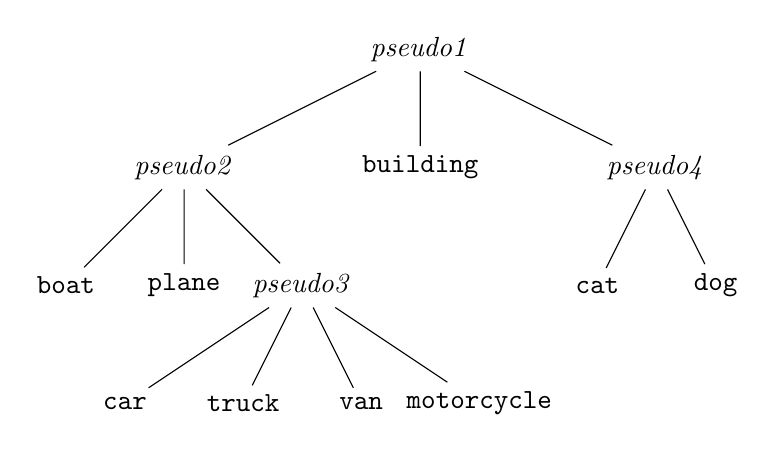
\begin{tikzpicture}
    [ level distance=1.5cm
    , level 1/.style={sibling distance=3cm}
    , level 2/.style={sibling distance=1.5cm}
    ]
\node {\textit{pseudo1}}
    child {node {\textit{pseudo2}}
      child {node {\texttt{boat}}}
      child {node {\texttt{plane}}}
      child {node {\textit{pseudo3}}
        child {node {\texttt{car}}}
        child {node {\texttt{truck}}}
        child {node {\texttt{van}}}
        child {node {\texttt{motorcycle}}}
      }
      }
    child {node {\texttt{building}}}
    child {node {\textit{pseudo4}}
      child {node {\texttt{cat}}}
      child {node {\texttt{dog}}}
    };
\end{tikzpicture}
\end{center}

We parameterize the weight vectors from the label tree as follows.
For each leaf node $i$ (equivalently for each class $i$),
we let the sequence $P_i$ denote the path from the leaf node to the root.
For example, using the label tree above,
we have

\begin{equation}
\begin{split}
    P_{\texttt{truck}} &= (\texttt{truck}, \textit{pseudo3}, \textit{pseudo2}, \textit{pseudo1} ) \\
    P_{\texttt{cat}} &= (\texttt{cat}, \textit{pseudo4}, \textit{pseudo1} )
\end{split}
\end{equation}

% \end{equation}

Next, we associate a vector $\vv_i$ to each leaf and internal node $i$ in the tree structure.
In particular, there is a there is a vector $\vv_i$ for each class and for each pseudo-class.
Finally, we reparameterize the weights for the softmax cross entropy loss as the sum of the vectors along the paths.
Specifically, we set the weight vector for class $j$ to be 
\begin{equation}
    \label{eq:covertree-reparam}
    \w_j = \sum_{k\in P_j} \vv_k
    .
\end{equation}
Substituting \eqref{eq:covertree-reparam} into \eqref{eq:xentropy} gives us the final cover tree loss
\begin{equation}
    \ell(V;(\x,y)) = - \log \frac {\exp(-\sum_{k\in P_y}\trans\vv_k \x)}{\sum_{j=1}^c \exp(- \sum_{k\in P_j}\trans\vv_k \x)}
\end{equation}
where $V=(\vv_1,...,\vv_k)$,
and our goal is to minimize $\ell$ with respect to $V$.
Note that this loss can easily be computed in libraries like pytorch or tensorflow with the standard cross entropy loss functions.
The only change needed is to define the loss in terms of the sum of vectors $V$ instead of a variable tensor $W$.

\subsection{Analysis}

When analyzing stochastic gradient descent using the cross entropy loss,
it is common to assume that the parameter space is bounded.
Under the standard parameterization, we have that the weight vector for each class satisfies $\ltwo{\w_j} \le B$.
It immediately follows that $\lF{W} \le \sqrt{c}B$,
and from this and convergence results of SGD it follows that the generalization error is $O(\sqrt{k}B/n)$.
(See Theorem \ref{theorem:xentropy} above.)

The key idea of the tree loss is that we can reduce the bound on the size of the parameter space,
and this will result in the reduced sample complexity.
Let $\level k$ denote the level of node $k$ in the label tree.
Then we replace the constraints on the $\w_j$s with the following constraint on all $\vv_k$:
\begin{equation}
    \ltwo{\vv_k} \le \frac{B}{2^{\level k}}
    .
    \label{eq:tree-constraint}
\end{equation}
Notice that the original constraint \eqref{} immediately follows from the tree constraint \eqref{eq:tree-constraint} and the reparameterization \eqref{eq:covertree-reparam}.
One way to interpret this is that we have ``factored out'' our bounds on the $\w_i$ into bounds on the smaller $\vv_k$ components,
and because the $\vv_k$ vectors are shared between classes,
we can reduce the overall bound.
The following lemma bounds the Frobenius norm of the weight matrix $V$.

\begin{lemma}
    Assume that the label tree has at most $q$ nodes per level and $r$ levels.
    Then,
    \begin{equation}
        \lF{V} \le \tfrac12 Bq c^{(1 - 1/\log_2 q)}
    \end{equation}
    In particular, if $q=2$, then
    \begin{equation}
        \lF{V} \le B,
    \end{equation}
    which is independent of the number of classes $c$.
\end{lemma}
\begin{proof}
    We have the following chain of inequalities
    \begin{align}
        \lF{V} 
        &\le \sum_{k\in \text{nodes of the level tree}} \ltwo{\vv_k}
        \\
        &= \sum_{i=0}^r \sum_{k\in \text{nodes at level $i$}} \ltwo{\vv_k}
        \\
        &\le \sum_{i=0}^r B\left(\frac {q} {2}\right)^i
        \label{eq:lem:lFV:1}
        \\
        &=
        B\left(\frac{1 - (q/2)^{r+1}}{1-q/2}\right)
        \label{eq:lem:lFV:2}
        \\
        &\le
        B(q/2)^{r+1}.
        \label{eq:lem:lFV:3}
    \end{align}
    Line \eqref{eq:lem:lFV:1} follows from the fact that the number of nodes at level $i$ in the tree is upper bounded by $q^i$ and the the maximum L2 norm of a vector at level $i$ in the tree is $B/2^i$,so the sum of all vectors at level $i$ is bounded by $B(q/2)^i$.
    Lines \eqref{eq:lem:lFV:2} and \eqref{eq:lem:lFV:3} are standard properties of geometric series.

    Next, we show that
    \begin{equation}
    \begin{split}
        \left(\frac q 2\right)^r
        &=
        \left(\frac q 2\right)^{\log_q n}\\
        &=
        \frac{n}{2^{\log_q n}}\\
        &=
        \frac{n}{2^{{\log_2 n}/{\log_2 q}}}\\
        &=
        \frac{n}{n^{1/\log_2 q}}\\
        &=
        n^{\left(1 - {1}/{\log_2 q}\right)}
        .
        \label{eq:lem:technical2}
    \end{split}
    \end{equation}
    Substituting \eqref{eq:lem:technical2} into \eqref{eq:lem:lFV:3} gives the stated result.
\end{proof}

Substituting this Lemma into the SGD bounds gives us our main theorem: 

\begin{theorem}
\label{theorem:xentropy}
% Assume that for all $i\in[n]$, $\ltwo{x_i} \le \rho$,
%     and that for each class $i\in[c]$, $\ltwo{\w_i}\le B$.
\fixme{Add assumptions.}
Assume that for all $i\in[n]$, $\ltwo{x_i} \le \rho$,
    and that for each class $i\in[c]$,  $\ltwo{\w _i} \le \frac{B}{2^{\level i}}$.
Then the parameter vector $\bar W$ estimated from one epoch of SGD satisfies
\begin{equation}
    \E L_D(\bar W) - L_D(W^*) \le \frac {B\rho}{\sqrt n}
    ,
\end{equation}
which is independent of the number of classes $c$.
\end{theorem}
%Let $\mathcal L$ be a metric space over the set of labels,
%and $\ddim$ be the doubling dimension of $\mathcal L$.
%Then we build a ``cover tree'' from the class labels that respects the metric structure.
%This cover tree will have exactly $c$ leaf nodes, one for each class label,
%and $O(c)$ internal nodes.
%Why does this small change work?
%Intuitively, classes that have a small distance from each other should have similar weight vectors.

%\begin{lemma}
    %Under the conditions defined above, we have
%\begin{equation}
    %\label{eq:lFV-bound}
    %\lF{V} \le (\ddim \log c) B.
%\end{equation}
%\end{lemma}
%\begin{proof}
%\end{proof}

%Formally, we can bound the Frobenius norm of the weight matrix $V$ by
%which is significantly better than our bound on the weight matrix $W$ of only $\sqrt c B$.
%Substituting \eqref{eq:lFV-bound} into Theorem 14.12 of Shalev-Shwartz and Ben-David gives us that if SGD is run for $T$ iterations to compute parameter estimate $\bar W$,
%then
%\begin{equation}
    %\E L_D(\bar W) - L_D(W^*) \le \frac {\sqrt {\dim \mathcal L}B\rho\log c}{\sqrt T}
%\end{equation}
%where $W^* = \argmin L_D(W)$.


\subsection{Bias-variance tradeoff}
\label{sec:bias-var}

\section{Experiments}

\subsection{Synthetic data}

In this experiment we will demonstrate the cover tree loss's effectiveness on a simple multiclass logistic regression problem.
The problem will be specifically designed to be convex and have low intrinsic dimension in the class labels in order to illustrate the advantages of the cover tree loss.

Let $N$ be the standard normal distribution.
Then sample the matrices
\begin{align}
    U \sim N^{c\times a} \qquad\text{and}\qquad
    A \sim N^{a\times d},
\end{align}
and define the true parameter matrix to be
\begin{equation}
    W^* = UA.
\end{equation}
For all $i \in [c]$, the row $\w_i^*$ of $W^*$ corresponds to the parameter vector for class $i$ and has dimension $d$.
The variable $a$ controls the intrinsic dimensionality of the problem.
When $a$ is small, then many class labels will be similar to each other;
but as $a$ increases, the class labels will have increasingly less structure.
When $a$ is known in advance, then we can use weight matrix factorization and set $e=a$.

For each data point $i\in[n]$,
we sample the data point according to the following rules:
\begin{align}
    y_i &\sim \text{Uniform}([c]), \text{and} \\
    \x_{i} &\sim \mathcal N(\w^*_{y_i}; \sigma),
\end{align}
where $\sigma$ controls the noise in the dataset.
Increasing $\sigma$ adds noise and makes classes harder to distinguish,
whereas decreasing $\sigma$ reduces noise and makes the classes easier to distinguish.

With our problem defined in this way, it is clear that
\begin{equation}
    \argmin_{W} \tfrac 1 n \ell(W; \x_i, y_i)
\end{equation}
converges to $W^*$ using the standard cross entropy loss and both the matrix factorization and cover tree reparameterizations.
% \fixme{You should prove this for yourself.}
% Figure \ref{fig:synthetic-results} shows that the cover tree loss converges at a faster rate.

\begin{figure*}
        \centering
        \begin{subfigure}[b]{0.45\textwidth}
            \centering
            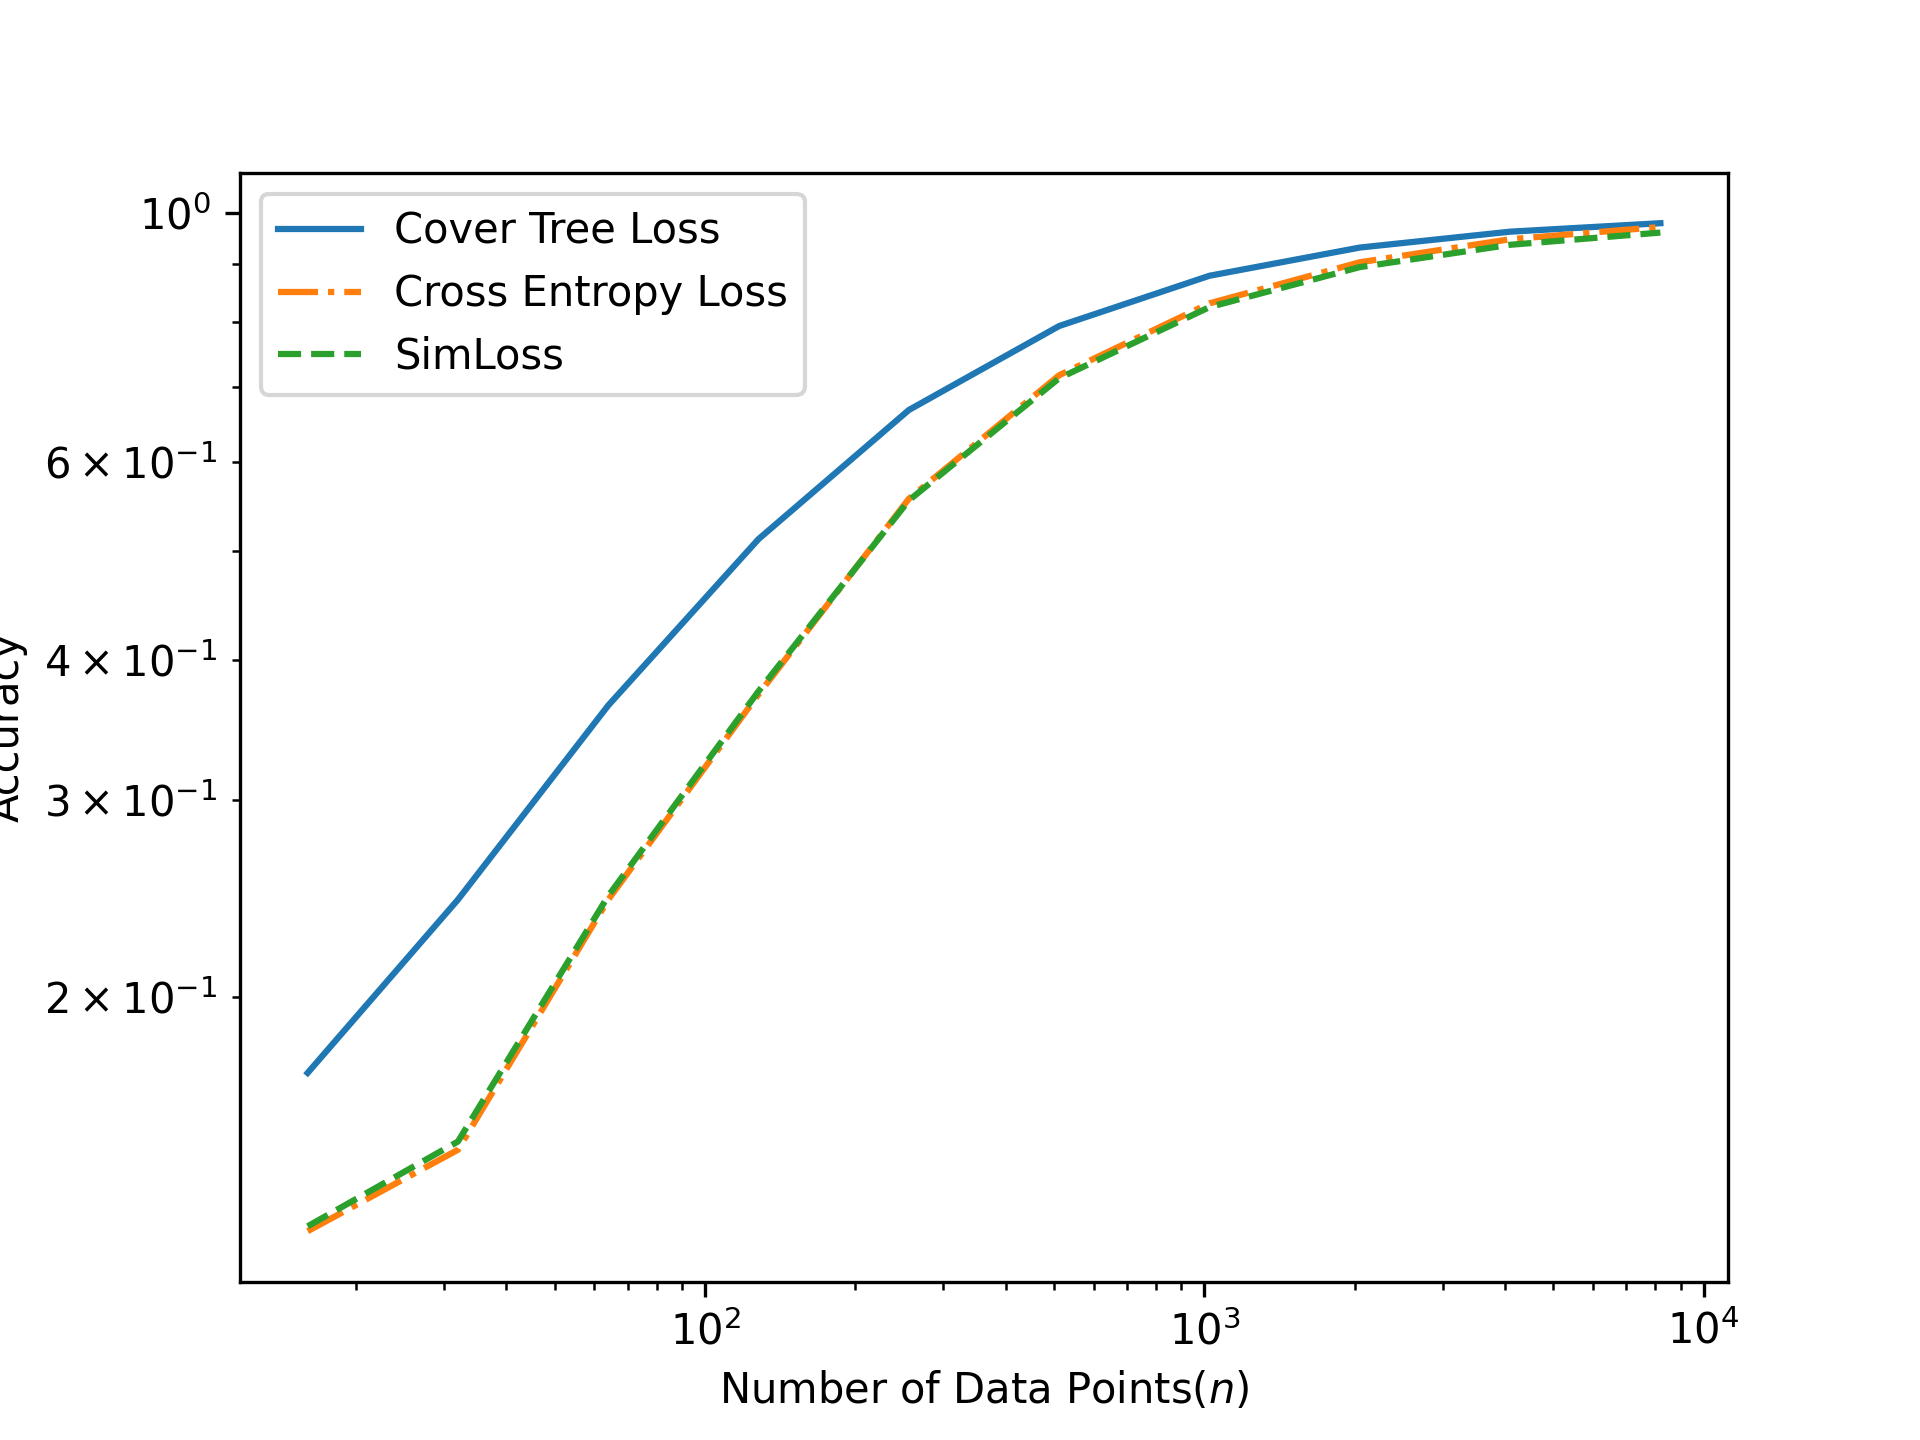
\includegraphics[width=\textwidth]{fig/images/accuracy_vs_n.png}
            % \caption[Accuracy versus number of data points($d=64, \sigma=1.0, c=10$)]%
            {{\small Accuracy versus number of data points($d=64, \sigma=1.0, c=10$)}}  
            \label{subfig.1}
        \end{subfigure}
        \hfill
        \begin{subfigure}[b]{0.45\textwidth}  
            \centering 
            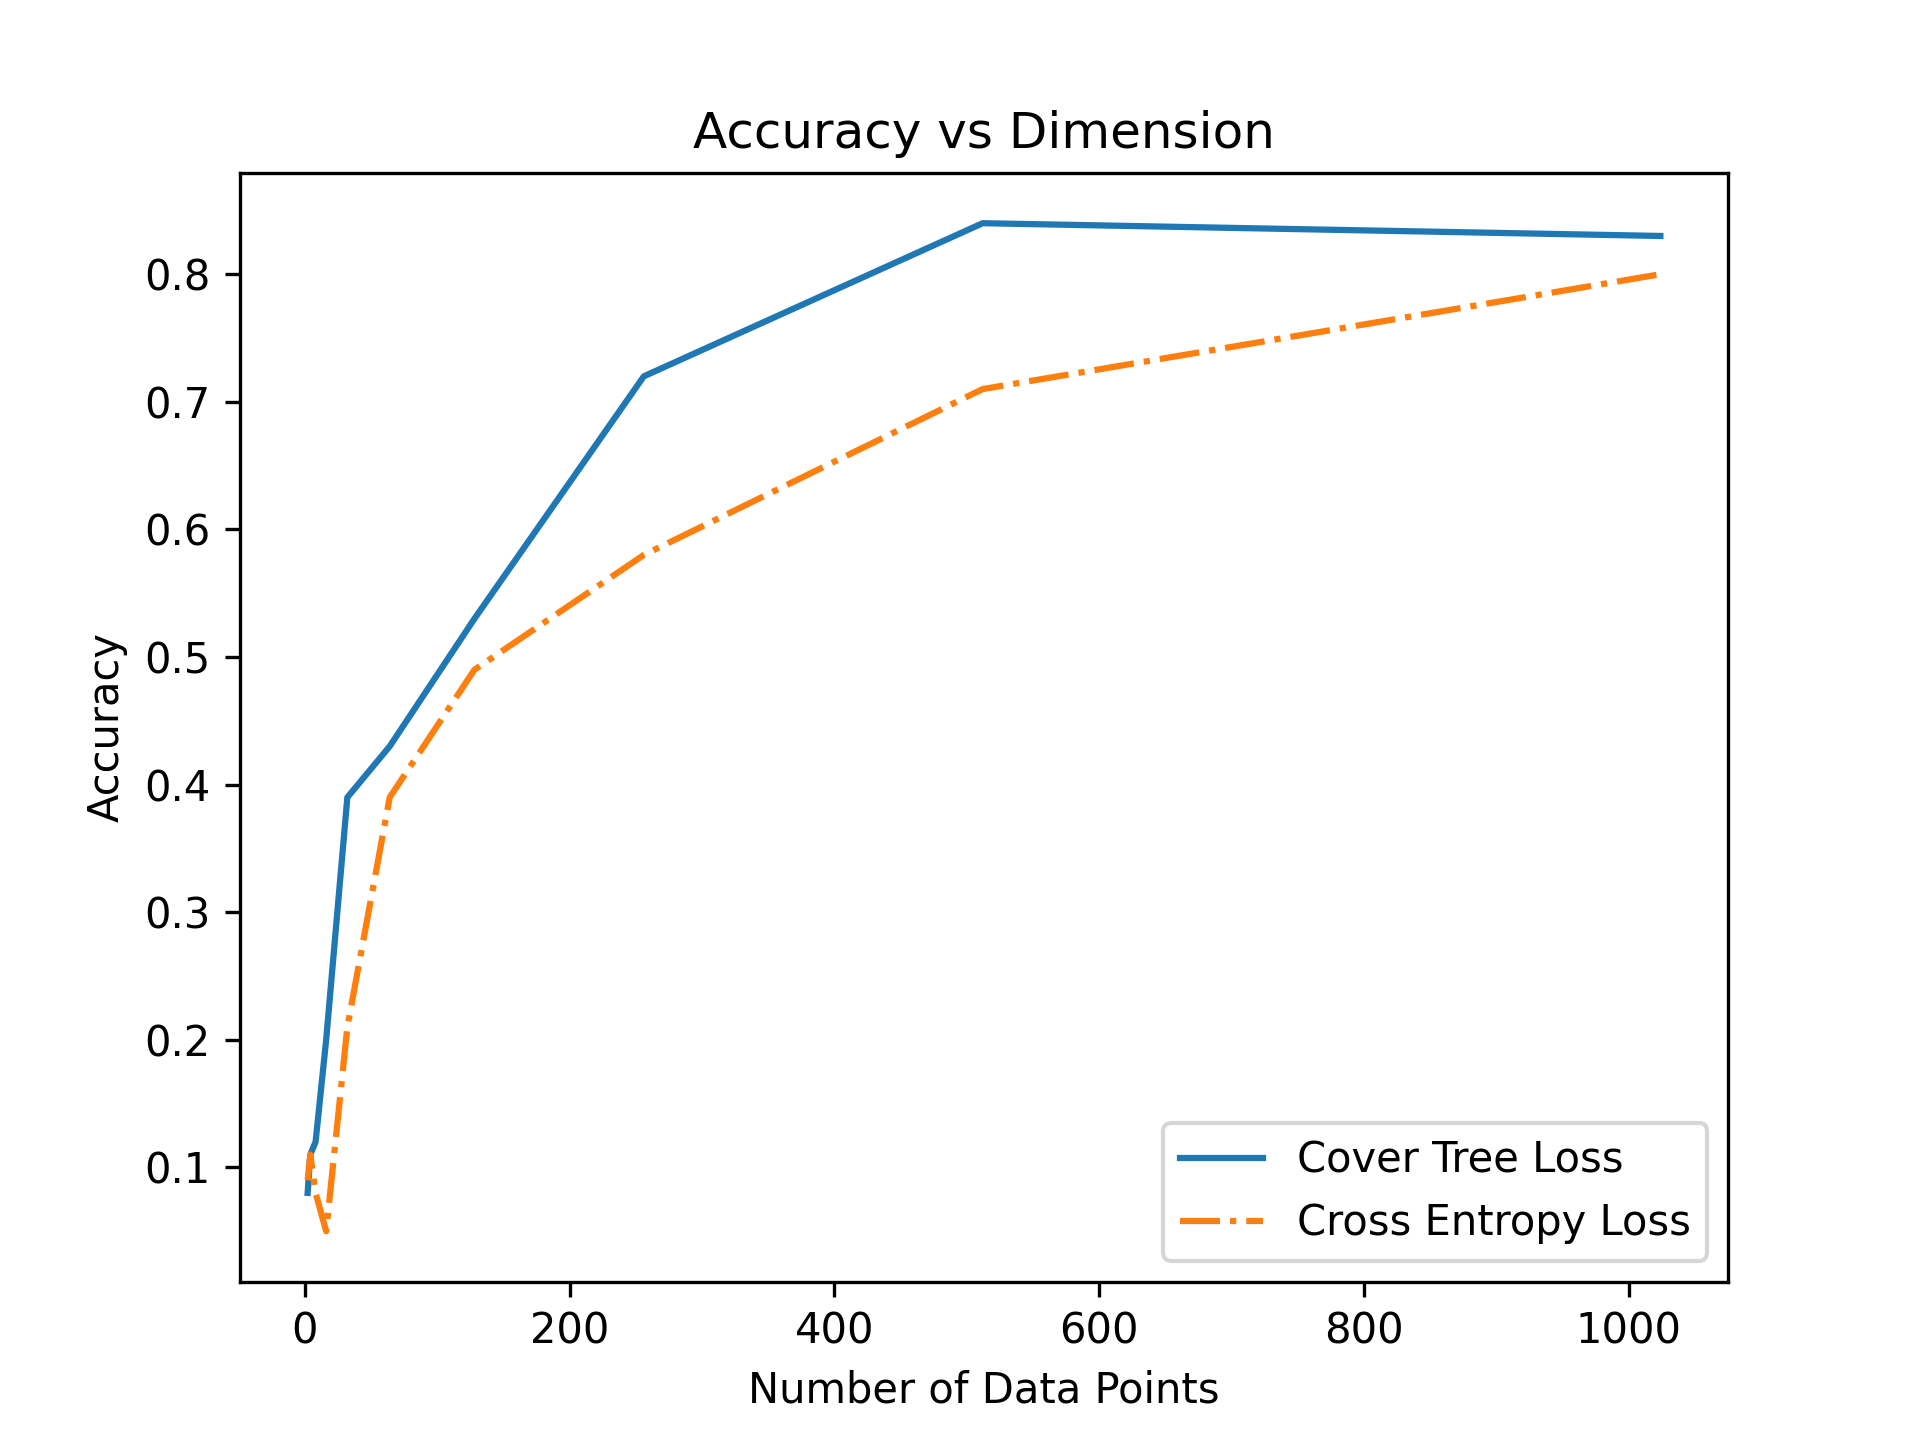
\includegraphics[width=\textwidth]{fig/images/accuracy_vs_d.png}
            % \caption[Accuracy versus dimension of parameter matrix($n=100, \sigma=1.0, c=10$)]%
            {{\small Accuracy versus dimension of parameter matrix($n=100, \sigma=1.0, c=10$)}}
            \label{subfig.2}
        \end{subfigure}
        \vskip\baselineskip
        \begin{subfigure}[b]{0.45\textwidth}   
            \centering 
            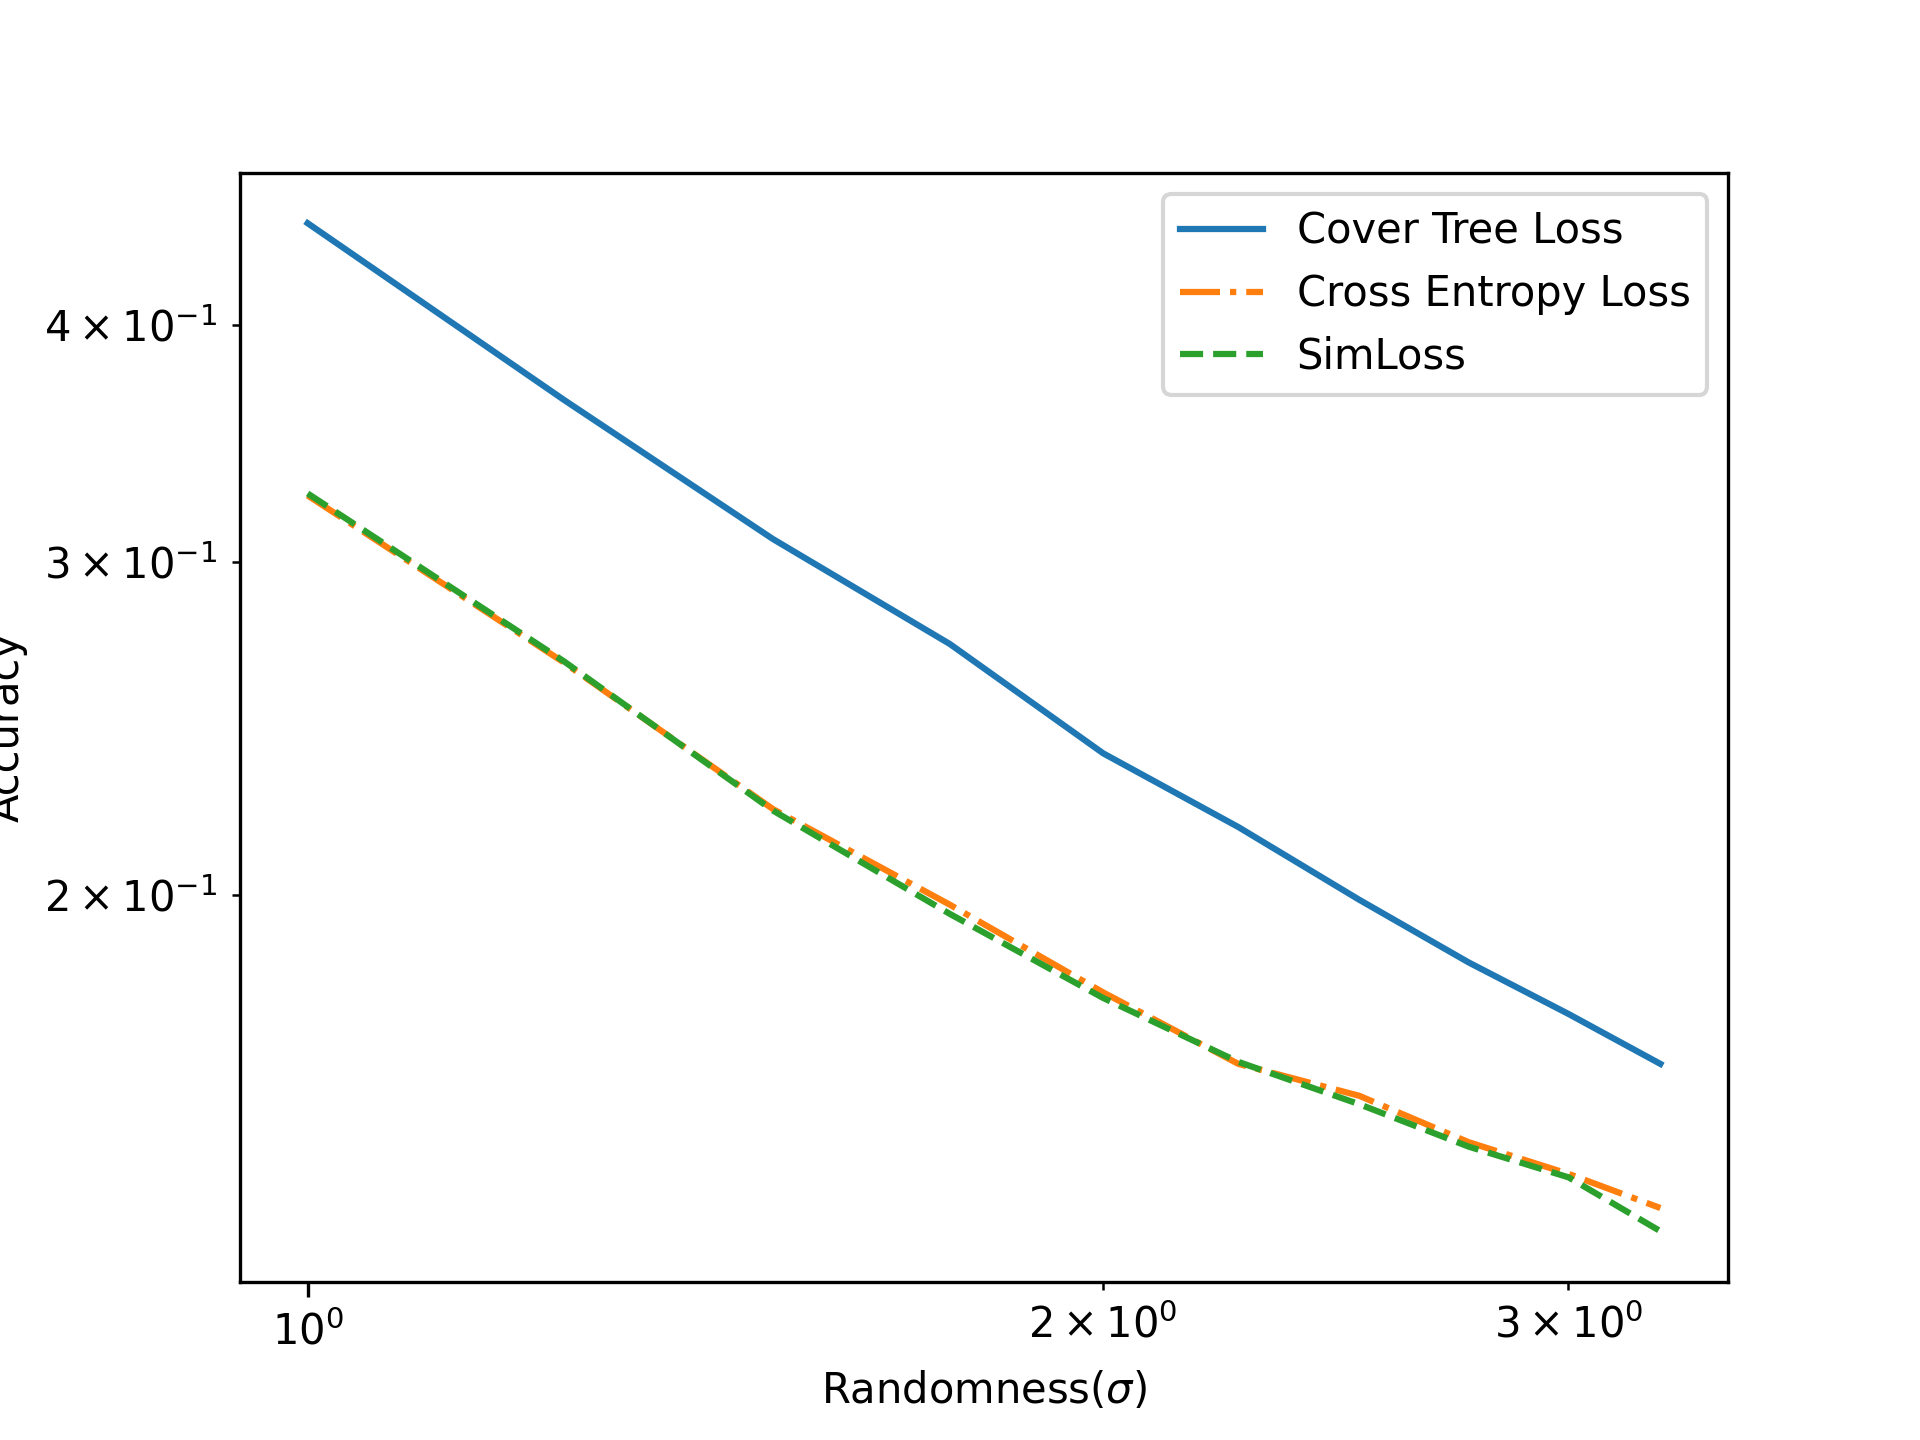
\includegraphics[width=\textwidth]{fig/images/accuracy_vs_sigma.png}
            % \caption[Accuracy versus randomness($n=100, d=64, c=10$)]%
            {{\small Accuracy versus randomness($n=100, d=64, c=10$)}}
            \label{subfig.3}
        \end{subfigure}
        \hfill
        \begin{subfigure}[b]{0.45\textwidth}   
            \centering 
            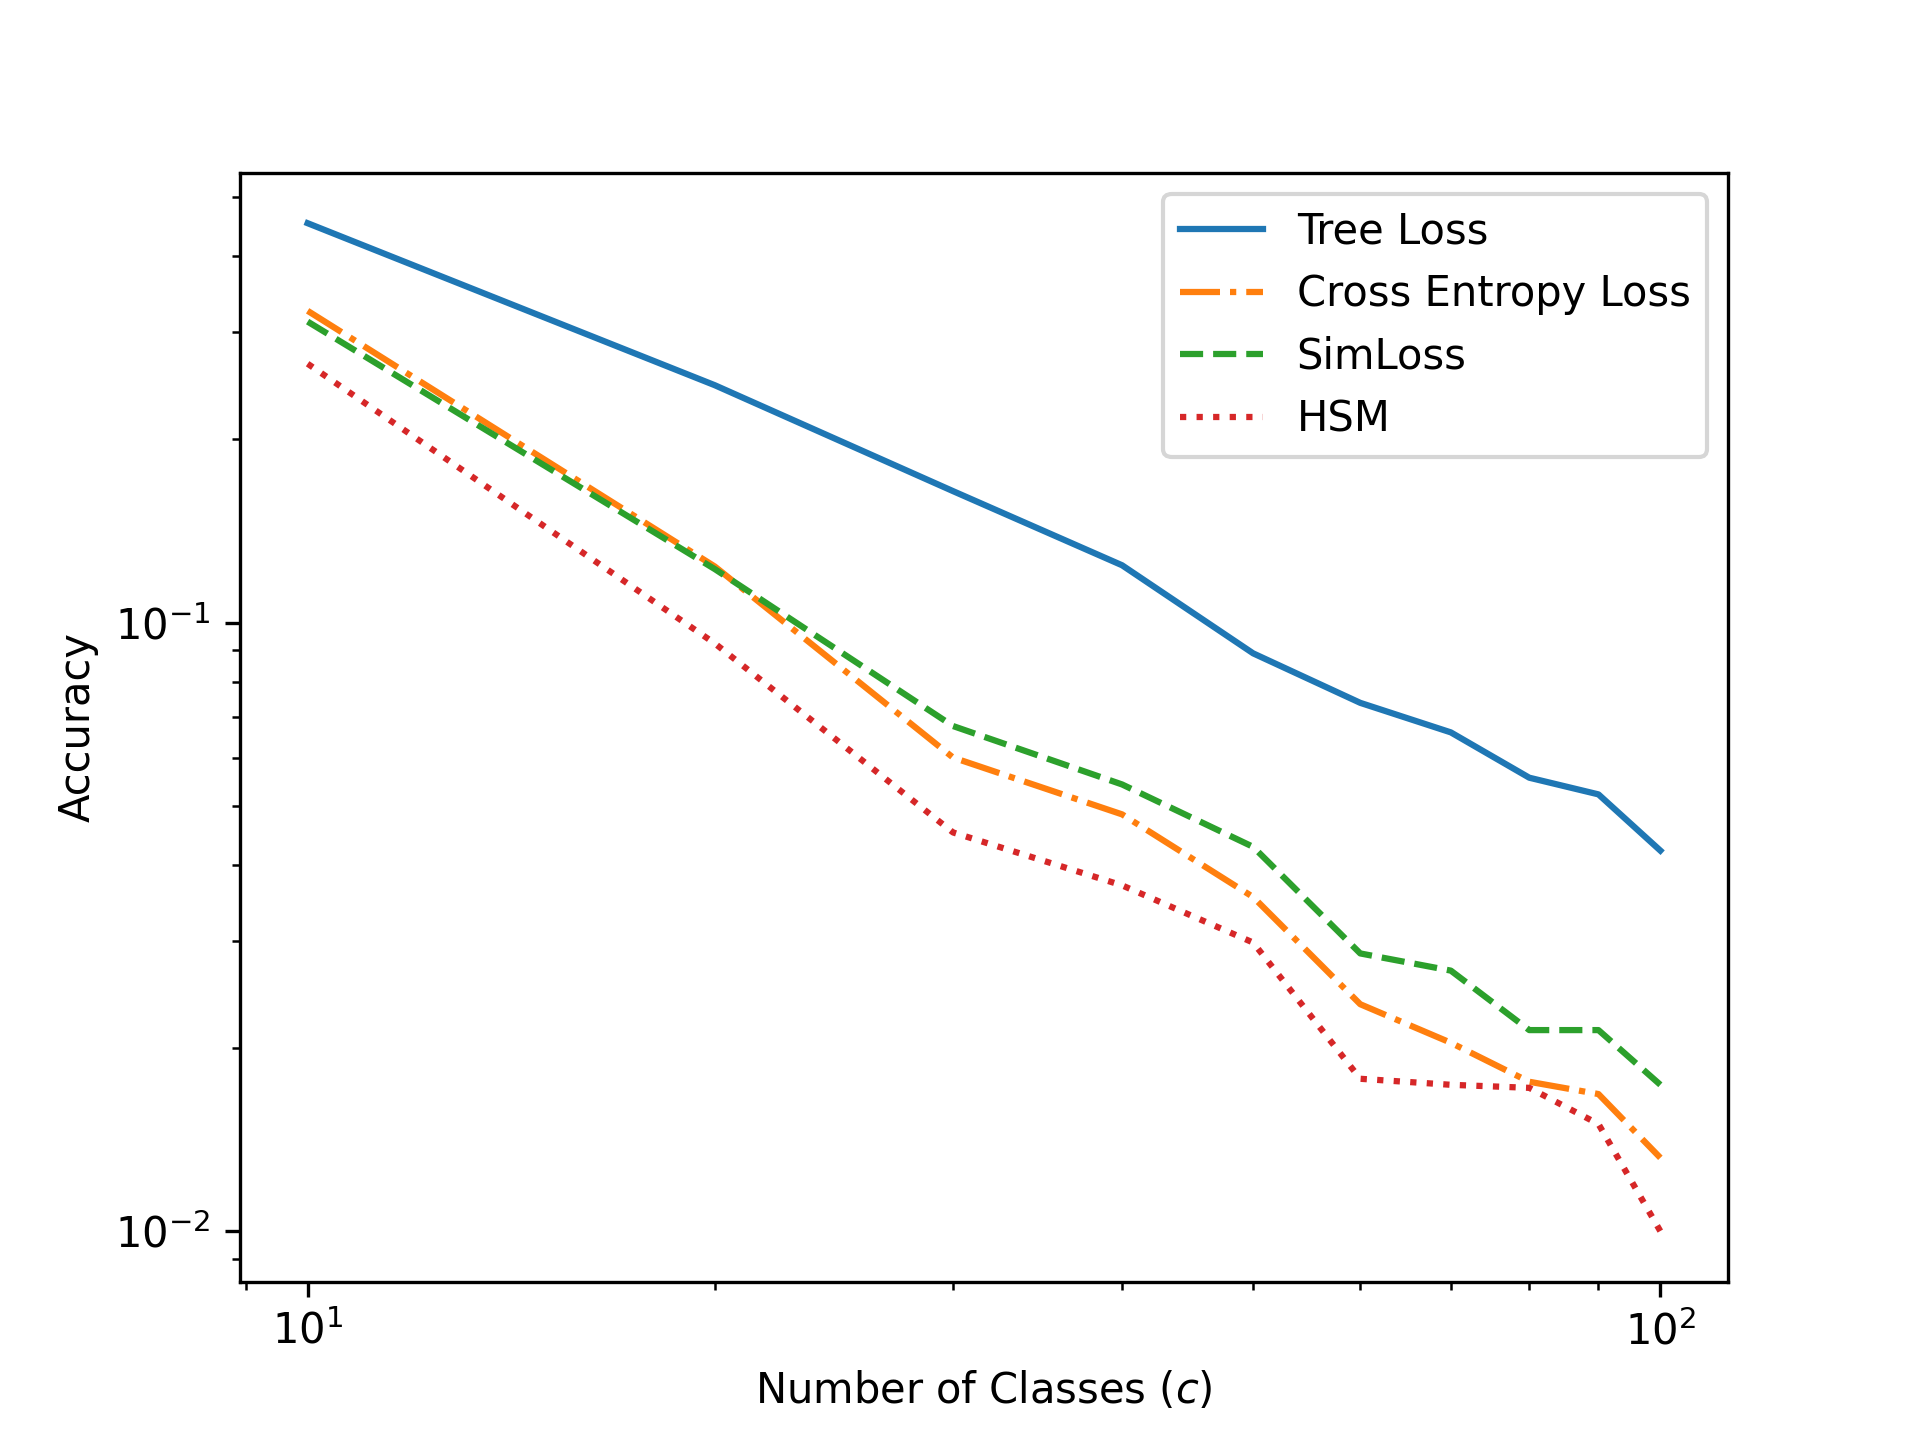
\includegraphics[width=\textwidth]{fig/images/accuracy_vs_class.png}
            % \caption[Accuracy versus number of classes($n=100, d=64, \sigma=1.0$)]%
            {{\small Accuracy versus number of classes($n=100, d=64, \sigma=1.0$)}}   
            \label{subfig.4}
        \end{subfigure}
        % \caption[ Figures of Synthetic Data Experiment ]
        % {{\small Figures of Synthetic Data Experiment}}
        \label{fig.1}
    \end{figure*}
    

\begin{figure*}
        \centering
        \begin{subfigure}[b]{0.45\textwidth}
            \centering
            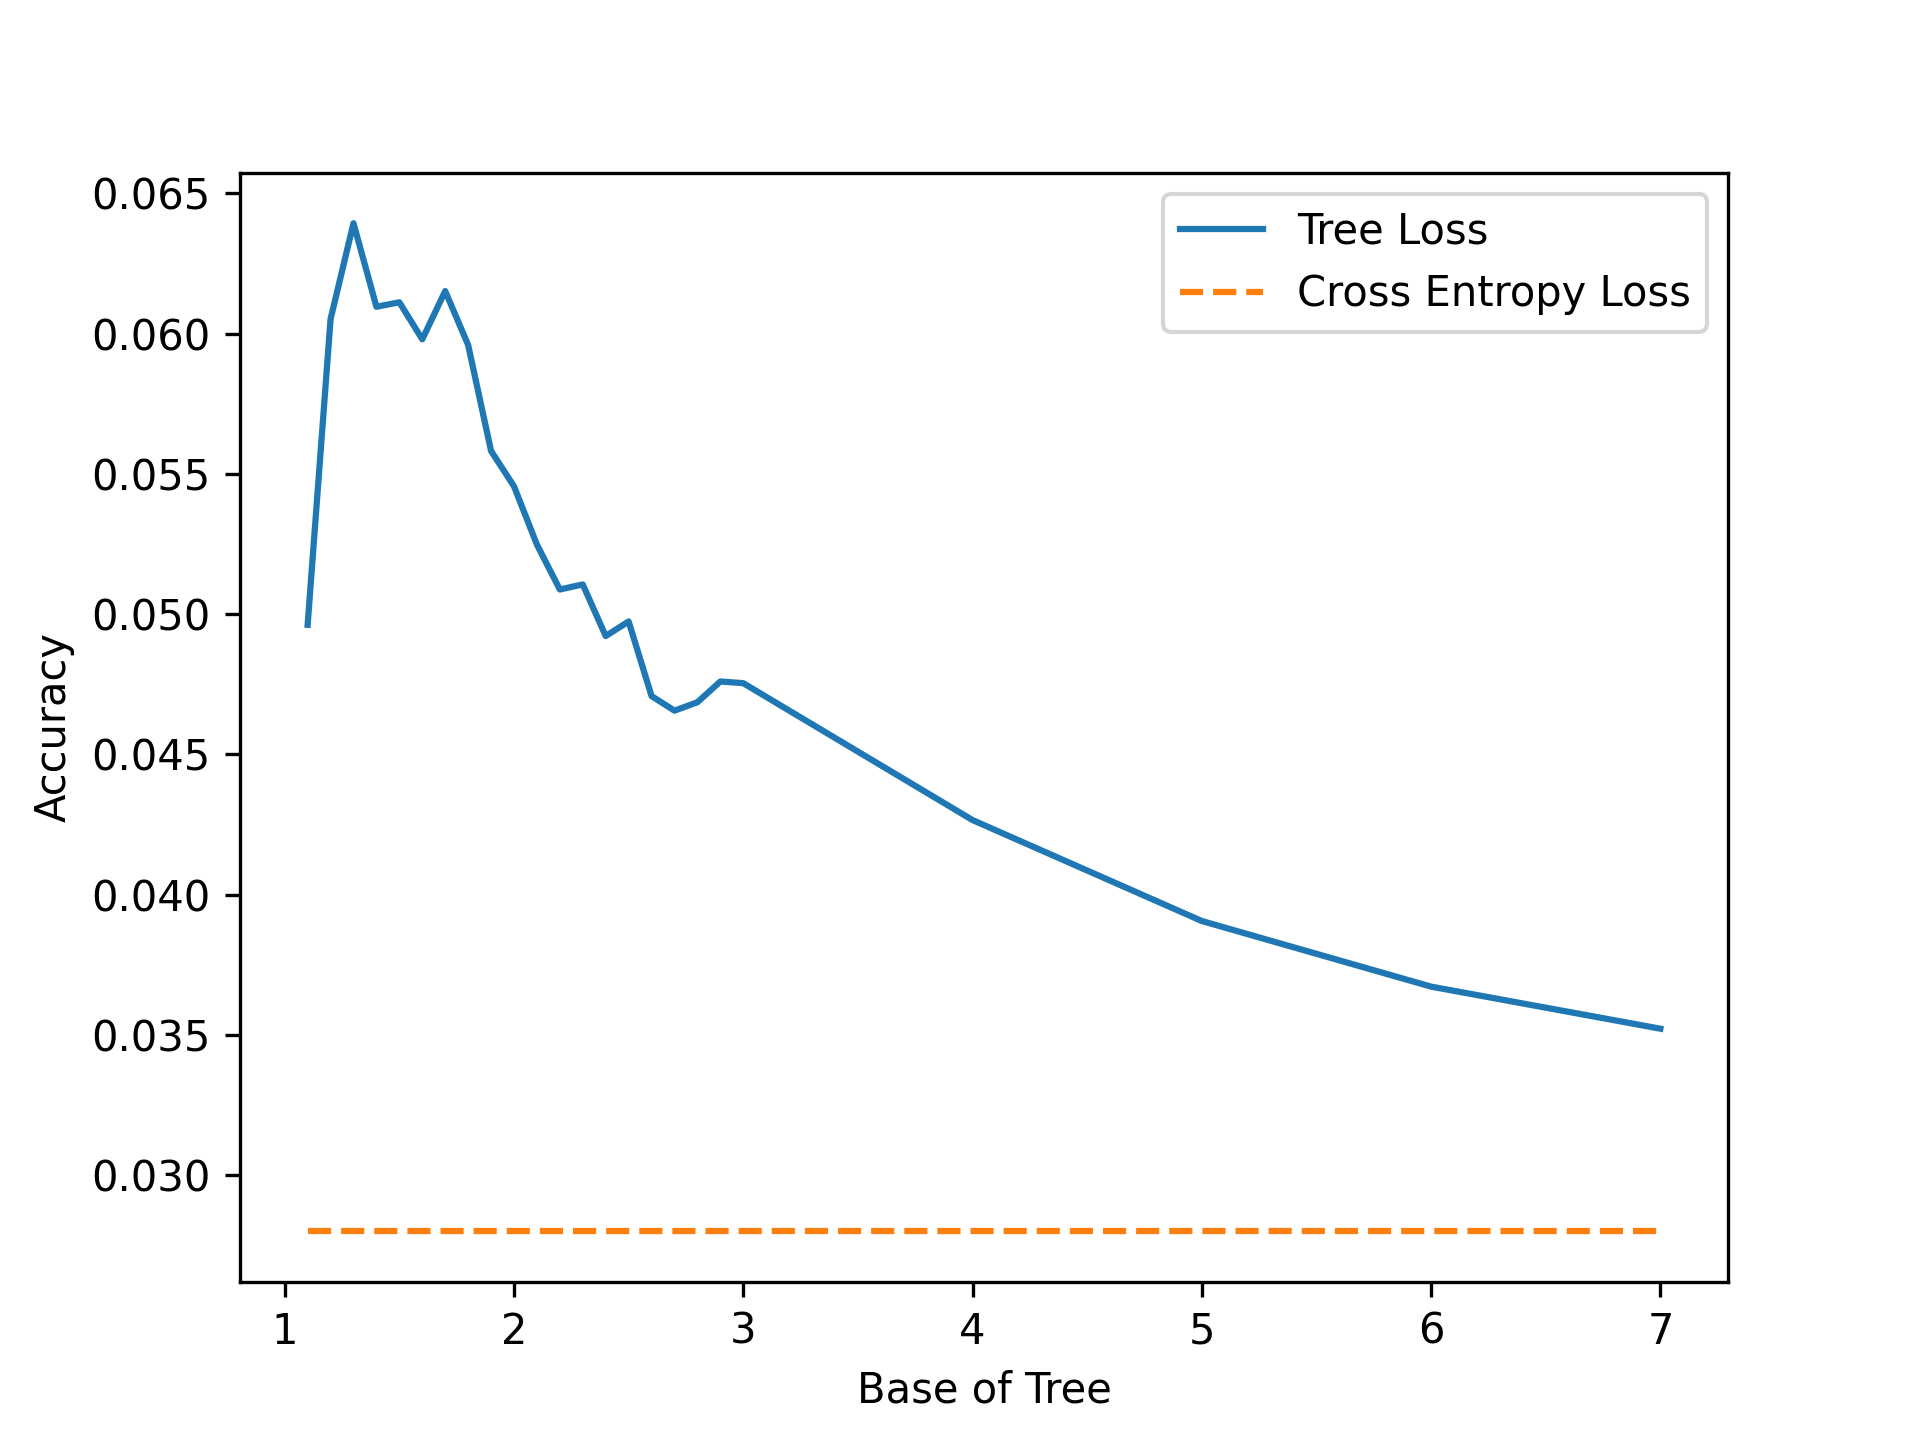
\includegraphics[width=\textwidth]{fig/new_img/accuracy_vs_base.png}
            {{\small Accuracy versus base of cover tree($n=1000, d=10, \sigma=1.0, c=100$)}}
            \label{subfig.1}
        \end{subfigure}
        \hfill
        \begin{subfigure}[b]{0.45\textwidth}  
            \centering 
            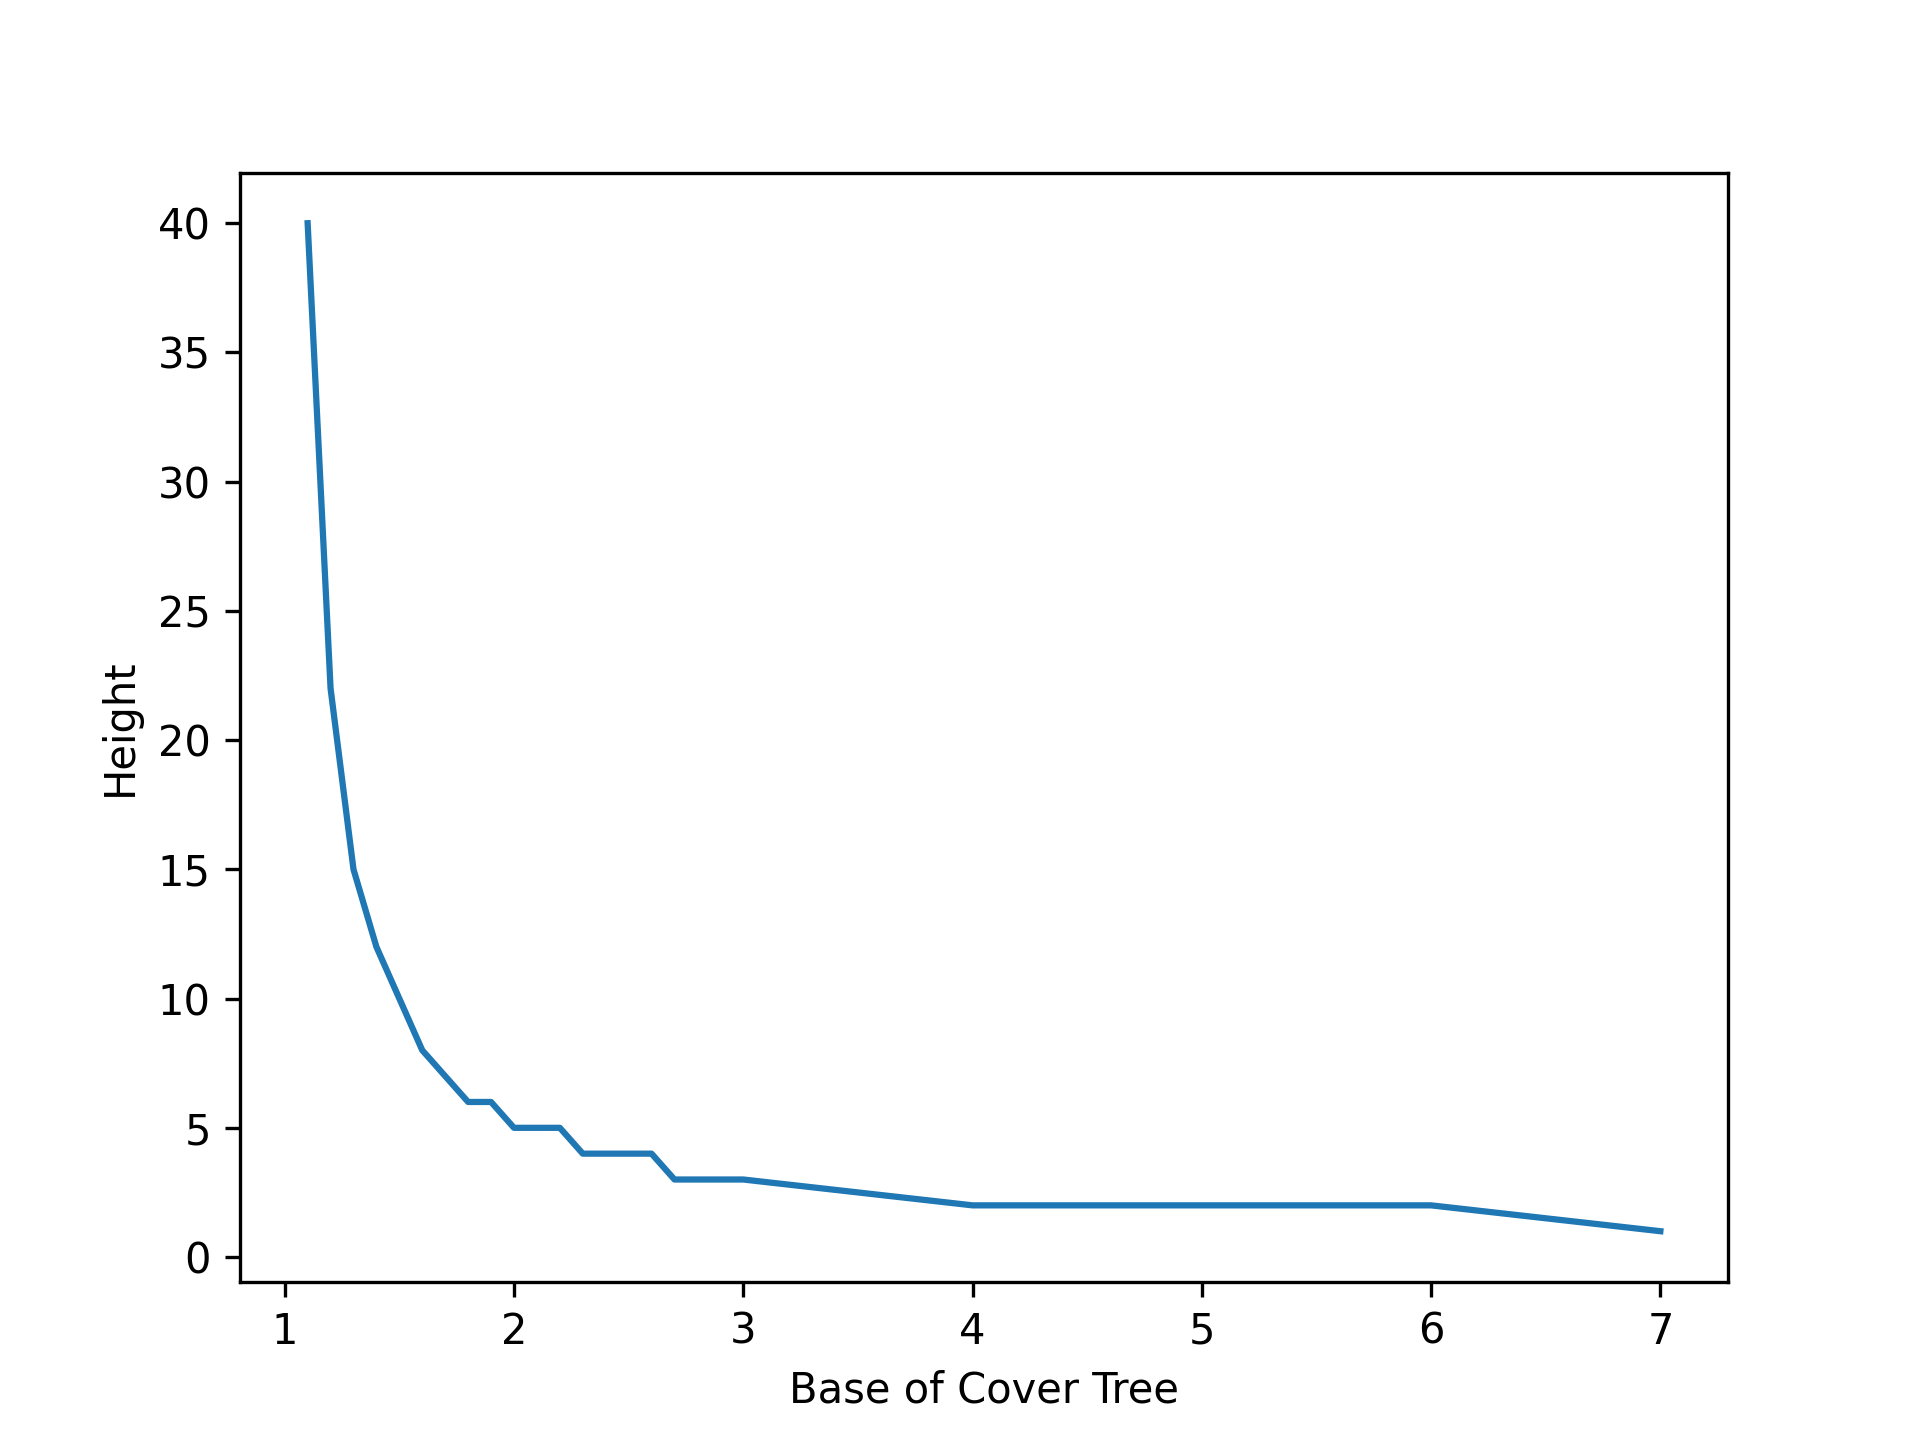
\includegraphics[width=\textwidth]{fig/new_img/height_vs_base.png}
            {{\small Height versus base of cover tree($n=1000, d=10, \sigma=1.0, c=100$)}}   
            \label{subfig.2}
        \end{subfigure}
        \vskip\baselineskip
        \begin{subfigure}[b]{0.45\textwidth}   
            \centering 
            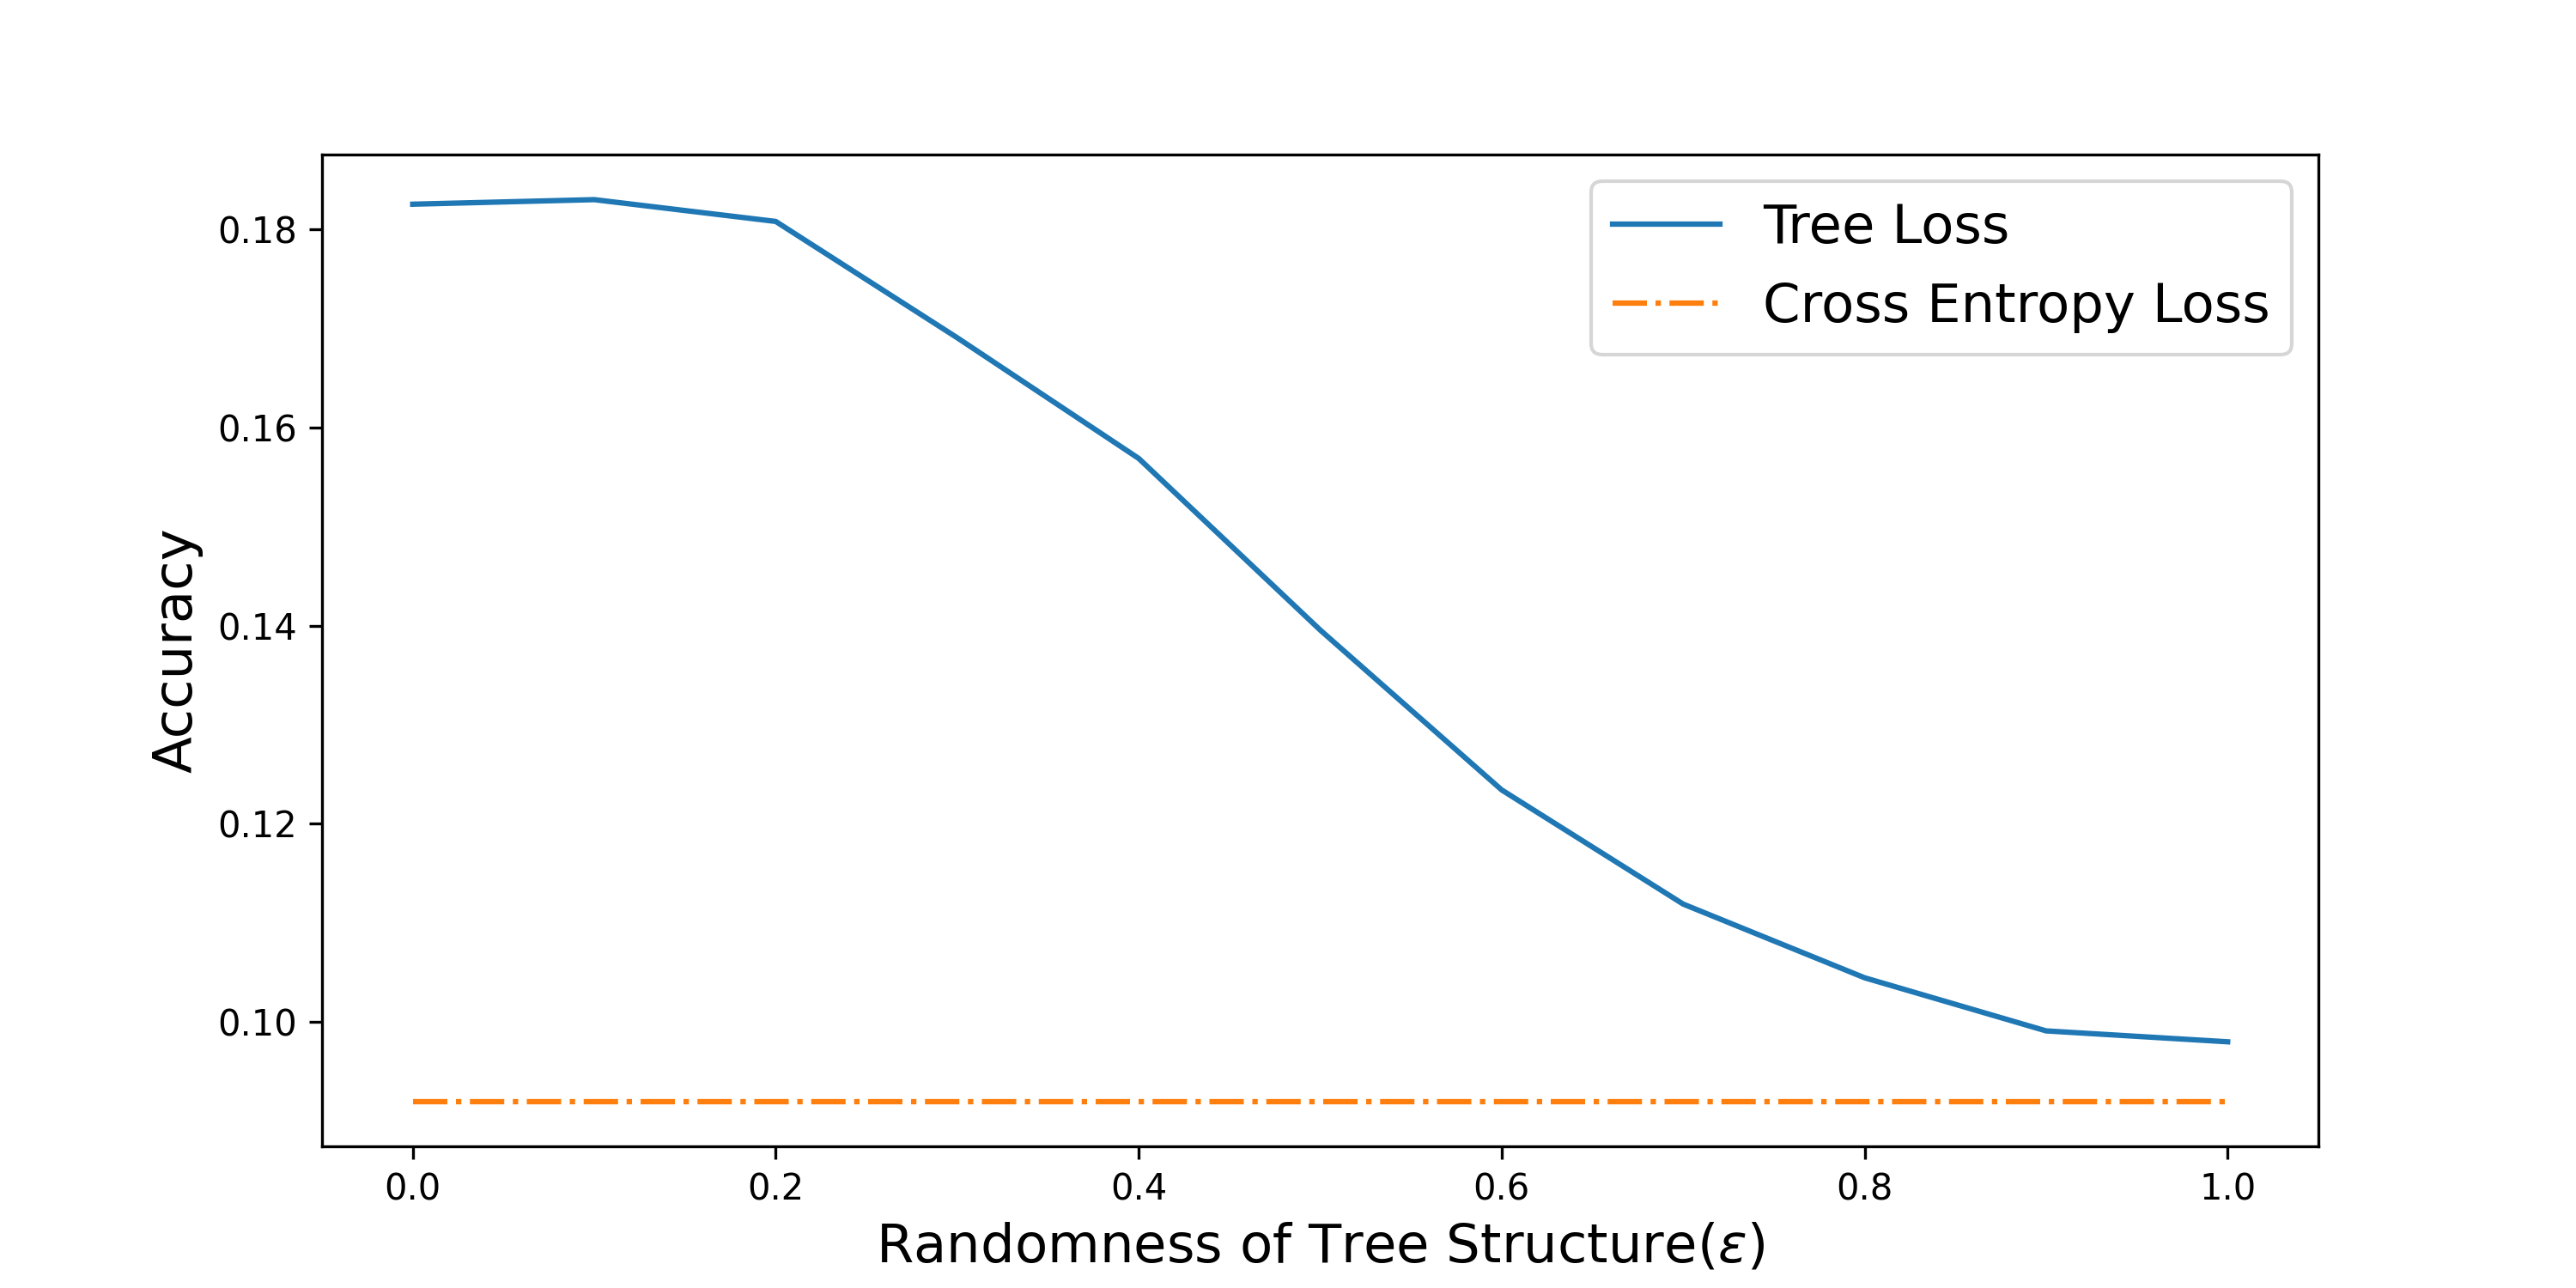
\includegraphics[width=\textwidth]{fig/new_img/loss_vs_structure.png}
            % \caption[Accuracy versus randomness($n=100, d=64, c=10$)]%
            {{\small Accuracy versus cover tree structure($n=1000, d=64, \sigma=1.0, c=100$)}}  
            \label{subfig.3}
        \end{subfigure}
        \hfill
        % \begin{subfigure}[b]{0.45\textwidth}   
        %     \centering 
        %     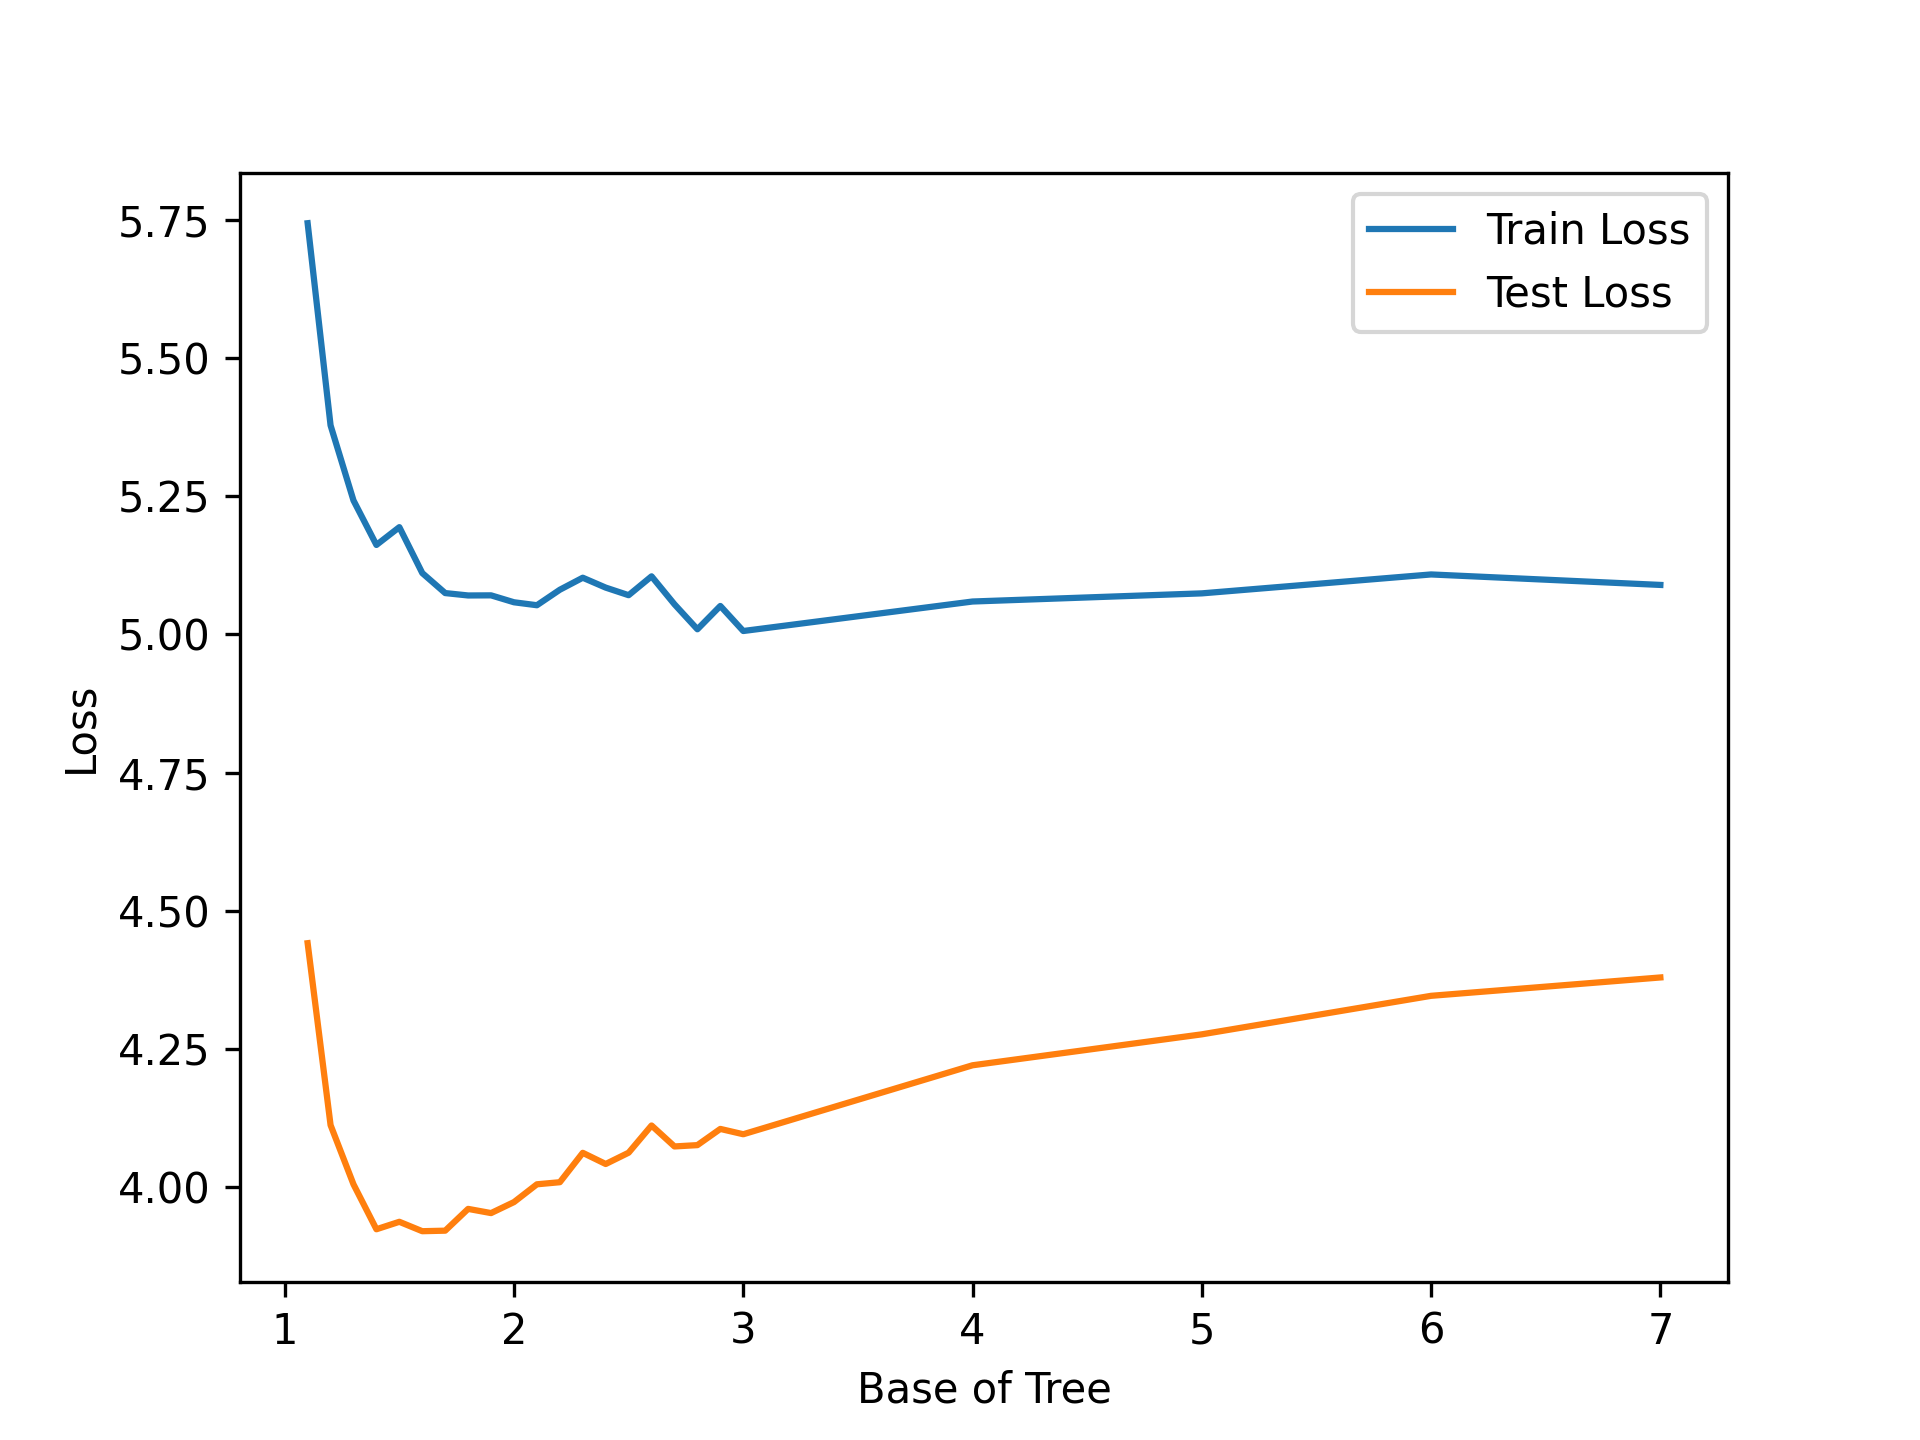
\includegraphics[width=\textwidth]{fig/new_img/loss_vs_base.png}
        %     % \caption[Accuracy versus number of classes($n=100, d=64, \sigma=1.0$)]%
        %     {{\small Loss versus base of cover tree($n=1000, d=10, \sigma=1.0, c=100$)}}    
        %     \label{subfig.4}
        % \end{subfigure}
        % \caption[ Figures of Synthetic Data Experiment ]
        % {{\small Figures of Synthetic Data Experiment}} 
        \label{fig.2}
    \end{figure*}


\subsubsection{Results}
From figure \ref{fig.1}, it is clear that the tree loss achieves the best performance. 
The tree loss converges at a faster rate as number of data points and dimension of parameter matrix increase.
If we increase the number of classes, the tree loss can keep a higher accuracy and the accuracy of SimLoss is higher than cross entropy loss and hierarchical softmax.
It is as our expected, the tree loss can improve performance on large classes tasks.
Besides, when we increase the noise in the dataset, the accuracy of all loss functions decrease, yet the tree loss decreases slower.
Among the four loss functions, hierarchical softmax hurts the performance obviously. 
We would not apply hierarchical softmax on real world data experiment in terms of computation.

There is a parameter 'base' which can control the height of tree.
Figure \ref{subfig.2} shows that if we increase the value of base, the tree is shorter.
As our expected, from figure \ref{subfig.1} we can see that a taller tree has higher accuracy. 
We add a parameter randomness into the tree structure and the tree structure become more random as the randomness factor increase.
As figure \ref{subfig.3} shows, when the tree structure become totally random, the performance of the tree loss is close to cross entropy loss.


\subsubsection{Alternative synthetic experiments}

In multi-label classification, it is common for the classes to be unbalanced.
We would like to show that the cover tree loss works well for unbalanced data.
A good way to do that is to change the distribution that $y_i$ is drawn from,
and a geometric distribution is a likely good alternative.

The cover tree loss can work well even when the weight matrix has non-linear intrinsic structure.
We should adapt the $\w*_i$ vectors to sit on a manifold instead of a hyperplane to demonstrate this fact.


\subsection{Real world data}
% \fixme{Write a description of the experiment.}
In this experiment, we will compare cover tree loss with softmax corss entropy and simloss on some real world data.
We conduct image classification tasks on CIFAR-100 dataset and ImageNet dataset and emoji prediction task on twitter dataset.
Our goal is to investigate the effects of changing the loss function on our example experiments.
We do not focus on if we have state-of-the-art performance on specific models, but rather on the evaluation of cover tree loss as a general loss function which can be applied on various tasks.
These three tasks and datasets are typical examples for using softmax cross entropy loss.

\subsubsection{CIFAR-100 Data}
We use CIFAR-100 dataset which has 100 classes for image classification.
We also get word embeddings from a word2vec model pretrained on Google News \cite{Mikolov2013EfficientEO} of class names and construct cover tree structure and calculate similarity between classes from word embeddings.
Four class names do not yield a word embedding and are therefore eliminated.

To evaluate our cover tree loss, we rely on three metrics: accuracy (Acc.) which focus on correct predictions and similarity accuracy (Similarity Acc.) which focus on the similarity of predicted and target class and superclass accuracy (SA). Every example in CIFAR-100 dataset has a main class and a superclass. Superclass accuracy is the fraction of examples that are correctly put into the corresponding superclass.
We take ResNet20 model \cite{He2016DeepRL} and SGD optimizer with a learning rate 0.1 and a batch size of 1021. 
We stop early to get the highest accuracy on validation set.


\begin{table}[]
\caption{Test results with early stopping on CIFAR-100 dataset. Best values are written in bold.} \label{cifar100}
\begin{center}
\begin{tabular}{@{}cccc@{}}
\toprule
\multirow{2}{*}{Loss} & \multicolumn{3}{c}{Test}    \\ \cmidrule(l){2-4} 
                      & Acc. & Similarity Acc. & SA \\ \cmidrule(r){1-1}
Tree Loss       & \textbf{52.78}     &  \textbf{65.90}               &  \textbf{62.55}  \\
Cross Entropy         &  51.87    &   65.58              &  62.14  \\
SimLoss               &    52.43  &    65.82             & 62.34  \\\bottomrule
\end{tabular}
\end{center}
\end{table}


\subsubsection{ImageNet Data}
ImageNet dataset \cite{Russakovsky2015ImageNetLS} has 1000 classes and many of the classes are similar and related, we consider the internal class structure has a impact on performance of loss function.
We use class names to get class representations from a pretrained FastText model.
We take ResNet50 model \cite{He2016DeepRL} trained on 1.28 mollion training images and evaluated on the 50k validation images and SGD optimizer with a learning rate 0.01.
We use top1 accuracy and top5 accuracy to evaluate our loss functions.



\begin{table}[]
\caption{Validation results on ImageNet dataset. Best values are written in bold.} \label{imagenet}
\begin{center}
\begin{tabular}{@{}ccc@{}}
\toprule
\multirow{2}{*}{Loss} & \multicolumn{2}{c}{Validation} \\ \cmidrule(l){2-3} 
                      & Top1 Acc.      & Top5 Acc.     \\ \cmidrule(r){1-1}
Tree Loss       & \textbf{76.52} & \textbf{92.92} \\
Cross Entropy         & 75.30          & 92.36         \\
SimLoss               & 76.24          & 92.83         \\ \bottomrule
\end{tabular}
\end{center}
\end{table}


\subsubsection{Twitter Data}

We apply the tree loss on emoji prediction in twitter dataset. 
Emojis are popular to express emotions in text messages and tweets are a wildely used social media over the world. 
We trained the multilingual BERT model on tweets to predict which emoji corresponds to a piece of text is best for measuring the emotional content in the text. 
Our 1660 target emojis are defined by emo2vec \cite{Eisner2016emoji2vecLE}.

We collect all tweets \cite{Izbicki2019GeolocatingTI} in any languages sent from anywhere in the world and filter the tweets with target emojis. 
For each tweet, we replace all user mentions with a special token \texttt{\text{<}mention\text{>}} and all URLS with a special token \texttt{\text{<}url\text{>}} and delete all emojis. 
We keep all hashtags and duplicate the tweet once for each emoji if a tweet has multiple emojis. 
Then we split the dataset into training validadtion and testing sets by user id to ensure each user appears in only one set in order to prevent data leakage.

We take the multilingual BERT model \cite{Feng2020LanguageagnosticBS} pretrained on data from 109 distinct languages which achieves state-of-the-art performance on a wide variety of natural language tasks. 
We get the embeddings of 1660 target emojis defined by emo2vec.

\begin{table}[h]
\small
\caption{Validation and test results of emoji prediction task on twitter dataset. Best values are written in bold.} \label{twitter}
\begin{center}
\begin{tabular}{@{}lcccc@{}}
\toprule
\multicolumn{1}{c}{\multirow{2}{*}{Loss}} & \multicolumn{2}{c}{VALIDATION} & \multicolumn{2}{c}{TEST}       \\ \cmidrule(l){2-5} 
\multicolumn{1}{c}{}                      & Acc.       & SA       & Acc.      & SA             \\ \cmidrule(r){1-1}
Tree Loss                           &   \textbf{20.81}    &   \textbf{50.26}  &  \textbf{20.96}    &   \textbf{50.45}        \\
Cross Entropy                             &   19.90    &   48.27  &  19.95    &   48.33        \\
SimLoss                                   &   19.91    &   48.25  &  19.96    &   48.32         \\ \bottomrule
\end{tabular}
\end{center}
\end{table}

\subsubsection{Results}
We evaluate the tree loss on image data(CIFAR100, ImageNet) and text data(Twitter) and the tree loss outperforms cross entropy loss and Simloss on metrics.
Table \ref{cifar100} shows the results of three loss functions for the test set of the CIFAR-100 dataset.
Similarity accuracy and superclass accuracy pay attention to more similar classes and the tree loss get higher accuracy.
Table \ref{imagenet} shows the results for the valdidation set of ImageNet dataset.
ImageNet has 1000 classes and many classes are semantically  similar.
The tree loss incorporates the similarities to training and get a higher top1 accuracy and top5 accuracy.
The emojis of Twitter dataset is typically unbalanced and the tree loss works well for unbalanced data.
Table \ref{twitter} shows the results for validation set and test set of twitter dataset.
The tree loss achieve the best performance on accuracy and similarity accuracy.


\section{Conclusion}
In this paper, we have presented the tree loss, a drop-in replacement for the cross entropy loss that incorporated class relations. 
We use properties of stochastic gradient descent to provide the theoretical justifications that the generalization error of the tree loss is better. 
The tree loss works by re-parameterizing the parameter matrix for softmax cross entropy loss and can be easily implement. 
We evaluate our tree loss on synthetic data and typically real world data. 
From the results of experiments, we found the tree loss improve the performance significantly and  help with predicting more similar classes if the model misclassified an example. 
In our analysis, since the tree loss can obtain background knowledge of classes, it works well for tasks with many classes and data with unbalanced classes. 


%%%%%%%%%%%%%%%%%%%%%%%%%%%%%%%%%%%%%%%%%%%%%%%%%%%%%%%%%%%%%%%%%%%%%%%%%%%%%%%%
\bibliographystyle{plainnat}
\bibliography{paper}
% \begin{abstract}
%   The Abstract paragraph should be indented 0.25 inch (1.5 picas) on
%   both left and right-hand margins. Use 10~point type, with a vertical
%   spacing of 11~points. The \textbf{Abstract} heading must be centered,
%   bold, and in point size 12. Two line spaces precede the
%   Abstract. The Abstract must be limited to one paragraph.
% \end{abstract}

% \section{GENERAL FORMATTING INSTRUCTIONS}

% The camera-ready versions of the accepted papers are 8 pages,
% plus any additional pages needed for references.

% Papers are in 2 columns with the overall line width of 6.75~inches (41~picas).
% Each column is 3.25~inches wide (19.5~picas).  The space
% between the columns is .25~inches wide (1.5~picas).  The left margin is 0.88~inches (5.28~picas).
% Use 10~point type with a vertical spacing of
% 11~points. Please use US Letter size paper instead of A4.

% Paper title is 16~point, caps/lc, bold, centered between 2~horizontal rules.
% Top rule is 4~points thick and bottom rule is 1~point thick.
% Allow 1/4~inch space above and below title to rules.

% Author descriptions are center-justified, initial caps.  The lead
% author is to be listed first (left-most), and the Co-authors are set
% to follow.  If up to three authors, use a single row of author
% descriptions, each one center-justified, and all set side by side;
% with more authors or unusually long names or institutions, use more
% rows.

% Use one-half line space between paragraphs, with no indent.

% \section{FIRST LEVEL HEADINGS}

% First level headings are all caps, flush left, bold, and in point size
% 12. Use one line space before the first level heading and one-half line space
% after the first level heading.

% \subsection{Second Level Heading}

% Second level headings are initial caps, flush left, bold, and in point
% size 10. Use one line space before the second level heading and one-half line
% space after the second level heading.

% \subsubsection{Third Level Heading}

% Third level headings are flush left, initial caps, bold, and in point
% size 10. Use one line space before the third level heading and one-half line
% space after the third level heading.

% \paragraph{Fourth Level Heading}

% Fourth level headings must be flush left, initial caps, bold, and
% Roman type.  Use one line space before the fourth level heading, and
% place the section text immediately after the heading with no line
% break, but an 11 point horizontal space.

% %%%
% \subsection{Citations, Figure, References}


% \subsubsection{Citations in Text}

% Citations within the text should include the author's last name and
% year, e.g., (Cheesman, 1985). 
% %Apart from including the author's last name and year, citations can follow any style, as long as the style is consistent throughout the paper.  
% Be sure that the sentence reads
% correctly if the citation is deleted: e.g., instead of ``As described
% by (Cheesman, 1985), we first frobulate the widgets,'' write ``As
% described by Cheesman (1985), we first frobulate the widgets.''


% The references listed at the end of the paper can follow any style as long as it is used consistently.

% %Be sure to avoid
% %accidentally disclosing author identities through citations.

% \subsubsection{Footnotes}

% Indicate footnotes with a number\footnote{Sample of the first
%   footnote.} in the text. Use 8 point type for footnotes. Place the
% footnotes at the bottom of the column in which their markers appear,
% continuing to the next column if required. Precede the footnote
% section of a column with a 0.5 point horizontal rule 1~inch (6~picas)
% long.\footnote{Sample of the second footnote.}

% \subsubsection{Figures}

% All artwork must be centered, neat, clean, and legible.  All lines
% should be very dark for purposes of reproduction, and art work should
% not be hand-drawn.  Figures may appear at the top of a column, at the
% top of a page spanning multiple columns, inline within a column, or
% with text wrapped around them, but the figure number and caption
% always appear immediately below the figure.  Leave 2 line spaces
% between the figure and the caption. The figure caption is initial caps
% and each figure should be numbered consecutively.

% Make sure that the figure caption does not get separated from the
% figure. Leave extra white space at the bottom of the page rather than
% splitting the figure and figure caption.
% \begin{figure}[h]
% \vspace{.3in}
% \centerline{\fbox{This figure intentionally left non-blank}}
% \vspace{.3in}
% \caption{Sample Figure Caption}
% \end{figure}

% \subsubsection{Tables}

% All tables must be centered, neat, clean, and legible. Do not use hand-drawn tables.
% Table number and title always appear above the table.
% See Table~\ref{sample-table}.

% Use one line space before the table title, one line space after the table title,
% and one line space after the table. The table title must be
% initial caps and each table numbered consecutively.

% \begin{table}[h]
% \caption{Sample Table Title} \label{sample-table}
% \begin{center}
% \begin{tabular}{ll}
% \textbf{PART}  &\textbf{DESCRIPTION} \\
% \hline \\
% Dendrite         &Input terminal \\
% Axon             &Output terminal \\
% Soma             &Cell body (contains cell nucleus) \\
% \end{tabular}
% \end{center}
% \end{table}

% \section{SUPPLEMENTARY MATERIAL}

% If you need to include additional appendices during submission, you can include them in the supplementary material file.
% You can submit a single file of additional supplementary material which may be either a pdf file (such as proof details) or a zip file for other formats/more files (such as code or videos). 
% Note that reviewers are under no obligation to examine your supplementary material. 
% If you have only one supplementary pdf file, please upload it as is; otherwise gather everything to the single zip file.

% You must use \texttt{aistats2022.sty} as a style file for your supplementary pdf file and follow the same formatting instructions as in the main paper. 
% The only difference is that it must be in a \emph{single-column} format.
% You can use \texttt{supplement.tex} in our starter pack as a starting point.
% Alternatively, you may append the supplementary content to the main paper and split the final PDF into two separate files.

% \section{SUBMISSION INSTRUCTIONS}

% To submit your paper to AISTATS 2022, please follow these instructions.

% \begin{enumerate}
%     \item Download \texttt{aistats2022.sty}, \texttt{fancyhdr.sty}, and \texttt{sample\_paper.tex} provided in our starter pack. 
%     Please, do not modify the style files as this might result in a formatting violation.
    
%     \item Use \texttt{sample\_paper.tex} as a starting point.
%     \item Begin your document with
%     \begin{flushleft}
%     \texttt{\textbackslash documentclass[twoside]\{article\}}\\
%     \texttt{\textbackslash usepackage\{aistats2022\}}
%     \end{flushleft}
%     The \texttt{twoside} option for the class article allows the
%     package \texttt{fancyhdr.sty} to include headings for even and odd
%     numbered pages.
%     \item When you are ready to submit the manuscript, compile the latex file to obtain the pdf file.
%     \item Check that the content of your submission, \emph{excluding} references, is limited to \textbf{8 pages}. The number of pages containing references alone is not limited.
%     \item Upload the PDF file along with other supplementary material files to the CMT website.
% \end{enumerate}

% \subsection{Camera-ready Papers}

% %For the camera-ready paper, if you are using \LaTeX, please make sure
% %that you follow these instructions.  
% % (If you are not using \LaTeX,
% %please make sure to achieve the same effect using your chosen
% %typesetting package.)

% If your papers are accepted, you will need to submit the camera-ready version. Please make sure that you follow these instructions:
% \begin{enumerate}
%     %\item Download \texttt{fancyhdr.sty} -- the
%     %\texttt{aistats2022.sty} file will make use of it.
%     \item Change the beginning of your document to
%     \begin{flushleft}
%     \texttt{\textbackslash documentclass[twoside]\{article\}}\\
%     \texttt{\textbackslash usepackage[accepted]\{aistats2022\}}
%     \end{flushleft}
%     The option \texttt{accepted} for the package
%     \texttt{aistats2022.sty} will write a copyright notice at the end of
%     the first column of the first page. This option will also print
%     headings for the paper.  For the \emph{even} pages, the title of
%     the paper will be used as heading and for \emph{odd} pages the
%     author names will be used as heading.  If the title of the paper
%     is too long or the number of authors is too large, the style will
%     print a warning message as heading. If this happens additional
%     commands can be used to place as headings shorter versions of the
%     title and the author names. This is explained in the next point.
%     \item  If you get warning messages as described above, then
%     immediately after $\texttt{\textbackslash
%     begin\{document\}}$, write
%     \begin{flushleft}
%     \texttt{\textbackslash runningtitle\{Provide here an alternative
%     shorter version of the title of your paper\}}\\
%     \texttt{\textbackslash runningauthor\{Provide here the surnames of
%     the authors of your paper, all separated by commas\}}
%     \end{flushleft}
%     Note that the text that appears as argument in \texttt{\textbackslash
%       runningtitle} will be printed as a heading in the \emph{even}
%     pages. The text that appears as argument in \texttt{\textbackslash
%       runningauthor} will be printed as a heading in the \emph{odd}
%     pages.  If even the author surnames do not fit, it is acceptable
%     to give a subset of author names followed by ``et al.''

%     %\item Use the file sample\_paper.tex as an example.

%     \item The camera-ready versions of the accepted papers are 8
%       pages, plus any additional pages needed for references.

%     \item If you need to include additional appendices,
%       you can include them in the supplementary
%       material file.

%     \item Please, do not change the layout given by the above
%       instructions and by the style file.

% \end{enumerate}

% \subsubsection*{Acknowledgements}
% All acknowledgments go at the end of the paper, including thanks to reviewers who gave useful comments, to colleagues who contributed to the ideas, and to funding agencies and corporate sponsors that provided financial support. 
% To preserve the anonymity, please include acknowledgments \emph{only} in the camera-ready papers.


% \subsubsection*{References}

% References follow the acknowledgements.  Use an unnumbered third level
% heading for the references section.  Please use the same font
% size for references as for the body of the paper---remember that
% references do not count against your page length total.

% \begin{thebibliography}{}
% \setlength{\itemindent}{-\leftmargin}
% \makeatletter\renewcommand{\@biblabel}[1]{}\makeatother
% \bibitem{} J.~Alspector, B.~Gupta, and R.~B.~Allen (1989).
%     \newblock Performance of a stochastic learning microchip.
%     \newblock In D. S. Touretzky (ed.),
%     \textit{Advances in Neural Information Processing Systems 1}, 748--760.
%     San Mateo, Calif.: Morgan Kaufmann.

% \bibitem{} F.~Rosenblatt (1962).
%     \newblock \textit{Principles of Neurodynamics.}
%     \newblock Washington, D.C.: Spartan Books.

% \bibitem{} G.~Tesauro (1989).
%     \newblock Neurogammon wins computer Olympiad.
%     \newblock \textit{Neural Computation} \textbf{1}(3):321--323.
% \end{thebibliography}

\end{document}
